% -*- TeX:UTF-8:Soft -*-

\documentclass[
	USenglish,12pt,paper=a4,numbers=noenddot,abstract=on,
	final,% remove sample info
	fullsample,
% 	centertables,
    ]{scrartcl}

\usepackage{pdflscape}

% !Mode:: "TeX:US:UTF-8:Soft"

% ********************************************************************
% Full Sample
% ********************************************************************
\def\pre{5p}
\def\preB{20p}

\newif\iffullsample
\DeclareOption{fullsample}{\fullsampletrue}\ProcessOptions*\relax
\iffullsample
\def\pre{100p}
\def\preB{100p}
\fi

\usepackage[scrtime]{prelim2e}
\renewcommand{\PrelimText}{\color{red}\footnotesize\textsf{\pre -sample} \textcolor{gray}{[\today -- \thistime]}}


% ********************************************************************
% Path to Figures
% ********************************************************************
\newcommand{\figpath}{}

\newif\ifneale
\DeclareOption{neale}{\nealetrue}\ProcessOptions*\relax
\ifneale
\renewcommand{\figpath}{}
\fi

\newif\ifjohn
\DeclareOption{john}{\johntrue}\ProcessOptions*\relax
\ifjohn
\renewcommand{\figpath}{}
\fi

\IfFileExists{C:/Dropbox/texlive/texmf-local/joerg.txt}{%
   \renewcommand{\figpath}{../../figures}%
}


% ***********************************
% Fonts & Language
% ***********************************
\usepackage[utf8]{inputenc}
\usepackage[T1]{fontenc}
% \usepackage{lmodern}
% \usepackage{amsmath}
% \usepackage{bm}
\usepackage{libertine}
\usepackage[libertine]{newtxmath}
\usepackage{microtype}
\usepackage{csquotes}
\usepackage{textcomp}
\usepackage{babel}

% ***********************************
% Useful Packages
% ***********************************
\usepackage{etoolbox}
\usepackage{xparse}
\usepackage{xpatch}

% ***********************************
% Page adjustments
% ***********************************
\usepackage{setspace}
\usepackage[normalsize,position=above,justification=centering]{caption}

\usepackage{geometry}
\geometry{paper=a4paper,left=2.5cm,right=2.5cm,top=2.5cm,bottom=2.5cm,footskip=30pt}

\setlength{\parindent}{2em}

\addtolength{\footnotesep}{.2\footnotesep}% increase space between footnotes
\deffootnote{0em}{0em}{\textsuperscript{\thefootnotemark}\hspace*{.3ex}}% footnotes to left text margin

\addtokomafont{disposition}{\rmfamily}
\addtokomafont{title}{\normalfont}
\setkomafont{author}{\large}
\setkomafont{date}{\large}
\setkomafont{section}{\large}
\setkomafont{subsection}{\normalsize}
\setkomafont{subsubsection}{\normalfont\normalsize\itshape}

% modify indent of titlepage footnotes
\makeatletter%
\patchcmd\maketitle{\@makefntext}{\@@@ddt}{}{}%
\patchcmd\maketitle{\rlap}{\mbox}{}{}%
\makeatother%

% Footnote without symbol with \fnsymbol[0]
\long\def\symbolfootnote[#1]#2{\begingroup%
   \def\thefootnote{\fnsymbol{footnote}}\footnote[#1]{#2}\endgroup}

\newcommand{\mail}[1]{\href{mailto:#1}{#1}}% Mail hyperlink

% Appendix
\usepackage{chngcntr}

\renewcommand{\appendix}{%
   \counterwithin{figure}{section}%
   \counterwithin{table}{section}%
   \renewcommand{\thesection}{\Alph{section}}%
   \renewcommand*{\thetable}{A\arabic{table}}%
   \renewcommand*{\thefigure}{A\arabic{figure}}%
   \setcounter{figure}{0}%
   \setcounter{table}{0}%
   % 	\section*{Appendix}%
   \phantomsection%
}

\frenchspacing%
\raggedbottom

% ********************************************************************
% Floats (Figure/Table placement)
% ********************************************************************
\usepackage[FIGTOPCAP]{subfigure}
\renewcommand{\thesubfigure}{(\Alph{subfigure})}
\renewcommand{\thesubtable}{(\Alph{subtable})}

\AtBeginEnvironment{table}{%
   \renewcommand{\subfigtopskip}{2.5ex}%
   \singlespacing
}

\usepackage{afterpage}
\usepackage{placeins}

\usepackage{floatpag}
\floatpagestyle{plain}

\usepackage{float}
\usepackage{rotfloat}
\rotfloatpagestyle{plain}
\usepackage{rotating}

\newenvironment{rotatepage}%
{\pagebreak[4]\global\pdfpageattr\expandafter{\the\pdfpageattr/Rotate 90}}%
{\pagebreak[4]\global\pdfpageattr\expandafter{\the\pdfpageattr/Rotate 0}}%

\BeforeBeginEnvironment{sidewaystable}{\begin{rotatepage}}
\AtBeginEnvironment{sidewaystable}{\floatplacement{table}{H}\singlespacing}
\AfterEndEnvironment{sidewaystable}{\end{rotatepage}}
\BeforeBeginEnvironment{sidewaysfigure}{\begin{rotatepage}}
\AtBeginEnvironment{sidewaysfigure}{\floatplacement{figure}{H}\singlespacing}
\AfterEndEnvironment{sidewaysfigure}{\end{rotatepage}}

% \AtBeginEnvironment{figure}{\singlespacing}

\newcommand{\ts}{\hspace{0.1cm} }
\newcommand{\vs}{\addlinespace}
\newcommand{\figwidth}{1\linewidth}


% subcaption
\newcounter{scaption}[figure]

\newcommand{\subcaption}[1]{%
	\stepcounter{scaption}%
	\medskip%
	\begin{minipage}[c]{\linewidth}%
	\centering\small%
	(\Alph{scaption}) #1%
	\smallskip%
	\end{minipage}%
}


% ***********************************
% Markings
% ***********************************
\usepackage[dvipsnames]{xcolor}

\usepackage{soulutf8}

\DeclareRobustCommand{\hllavender}[1]{{\sethlcolor{Lavender}\hl{#1}}}
\newcommand{\JW}[1]{\noindent\textsf{\hllavender{\textbf{JW}: #1}}}
\DeclareRobustCommand{\hlgreen}[1]{{\sethlcolor{green}\hl{#1}}}
\newcommand{\NM}[1]{\noindent\textsf{\hlgreen{\textbf{NM}: #1}}}
\DeclareRobustCommand{\hlcyan}[1]{{\sethlcolor{cyan}\hl{#1}}}
\newcommand{\JG}[1]{\noindent\textsf{\hlcyan{\textbf{JG}: #1}}}

% ********************************************************************
% Lists
% ********************************************************************
\usepackage{enumitem}
\setlist{%
   noitemsep,%
   topsep=0pt,%
   parsep=0pt,%
   partopsep=0pt,%
}

\renewcommand\labelitemi{--}
\renewcommand\labelitemii{\textbullet}


% ***********************************
% (Cross)References & Bibliography
% ***********************************
\usepackage[pdftex]{hyperref}
\hypersetup{colorlinks, citecolor=black, filecolor=black, linkcolor=black, urlcolor=black}

\usepackage[capitalise,nameinlink,noabbrev]{cleveref}%% clever ref; automatically adds "Figure," "Table," etc. when cross-ref. Need to place this after hyperref.
\creflabelformat{equation}{#2\textup{#1}#3}%
\AtBeginDocument{\let\ref\cref}

\usepackage{natbib}

\let\cite\citet


% ********************************************************************
% Crop PDF
% ********************************************************************
\let\oldincludegraphics\includegraphics

\makeatletter
\newcommand{\includecrop}[2][]{%
   \begingroup%
   \edef\temp@mdfivesum{\pdf@filemdfivesum{#2.pdf}}%
   \ifcsstrequal{#2mdfivesum}{temp@mdfivesum}{}{%
      %file changed
      \immediate\write18{pdfcrop #2 #2-crop.pdf}}%
   \immediate\write\@auxout{\string\expandafter\string\gdef\string\csname\space #2mdfivesum\string\endcsname{\temp@mdfivesum}}%
   \oldincludegraphics[#1]{#2-crop.pdf}%
   \endgroup%
}
\makeatother

\newif\ifpdfcrop%
\DeclareOption{pdfcrop}{\pdfcroptrue}\ProcessOptions*\relax%
\ifpdfcrop%
\let\includegraphics\includecrop%
\fi

% -*- TeX:UTF-8:Soft -*-

% ********************************************************************
% Necessary Packages
% ********************************************************************
\usepackage{xpatch}% for table line numbers patch
\usepackage{etoolbox}% for BeforeBeginEnvironment
\usepackage{xparse}% for \NewDocumentCommand
\usepackage{setspace}
\usepackage{multirow}
\usepackage{booktabs}
\usepackage{ragged2e}% for justify in fignote

% ********************************************************************
% siunitx
% ********************************************************************

% New \sym command. The stars themselves take no space, the box
% is set at the width of 888 (really only makes sense with T-OSF!
\NewDocumentCommand{\sym}{m}{\rlap{\text{#1}}\hphantom{888}}

\usepackage{siunitx}
\sisetup{% normal settings. Space for symbols then hooked in at econtables
   mode                    = text,
   group-digits            = false,
   input-symbols           = ( ) [ ] - +,
   table-space-text-post   = ,
   table-align-text-post   = false,
   input-signs             = ,
   table-number-alignment  = center
}

\AtBeginEnvironment{econtable}{\sisetup{table-space-text-post   = \sym{***}}}


% ********************************************************************
% estauto/estwide
% ********************************************************************

% \supersloppy ignores basically all \hbox errors.
% Fine for estout tables, but some side-effects possible,
% so a star version is softer.
\ProvideDocumentCommand\supersloppy{s}{%
   \IfBooleanTF#1%
   {\hfuzz=\maxdimen}%
   {\hfuzz=\maxdimen\tolerance=10000\hbadness=10000}%
}

% Create new etabular environments which ignore bad boxes
% Required to hook-into threeparttable
\newenvironment{etabular}%
{\supersloppy\tabular}%
{\endtabular\fussy}
\newenvironment{etabular*}%
{\supersloppy\begin{tabular*}}%
{\end{tabular*}\fussy}

\NewDocumentCommand{\estauto}{ m D<>{} m }{%
   \vspace{.75ex}{%
      \begin{etabular}{#1}%
         #2% Text before the top rule
         \toprule%
         #3%
         \bottomrule%
         \addlinespace[.75ex]%
      \end{etabular}
   }
}

\NewDocumentCommand{\estwide}{ O{1\textwidth} m D<>{} m }{%
   \vspace{.75ex}{%
      \begin{etabular*}%
         {#1}{@{\hskip\tabcolsep\extracolsep\fill}#2}%
         #3% Text before the top rule
         \toprule%
         #4%
         \bottomrule%
         \addlinespace[.75ex]%
      \end{etabular*}%
   }%
}


% ********************************************************************
% econtable
% ********************************************************************
\usepackage[para,flushleft]{threeparttablex}
\usepackage[export]{adjustbox}

% econtable uses always singlespacing, centering, adjustbox, threeparttable
\newenvironment{econtable}[1][tbp]%
{\begin{table}[#1]\begin{spacing}{1}\centering\adjustbox{center}\bgroup\begin{threeparttable}}%
{\end{threeparttable}\egroup\end{spacing}\end{table}}

\newenvironment{econlongtable}%
{\begin{ThreePartTable}%
   \RenewDocumentCommand{\estauto}{ m D<>{} m }{%
      \vspace{.75ex}{%
         \begin{longtable}{##1}%
            ##2% Text before the top rule
            \toprule%
            ##3%
            \bottomrule%
            \addlinespace[.75ex]%
         \end{longtable}%
      }%
   }%
   \def\estwide{\typeout{ERROR: command estwide is not defined for longtables}}%
   \renewcommand{\caption}[1]{\captionof{table}{##1}\vspace{-1\baselineskip}}%
   \setlength{\LTleft}{-20cm plus -1fill}\setlength{\LTright}{\LTleft}\begin{spacing}{1}}%
{\end{spacing}\end{ThreePartTable}}

\newcommand{\tabheader}[1]{#1}% command for the header that should be repeated of a longtable

%% Need to hook in etabular to threeparttable, otherwise \supersloppy has no effect
\makeatletter
\catcode`\*=11
\xpatchcmd{\threeparttable}
{\TPT@hookarg{tabularx}}
{\TPT@hookarg{tabularx}\TPT@hookin{etabular}\TPT@hookarg{etabular*}\supersloppy}
{}{}
\catcode`\*=12
\makeatother

% - To be on the safe side: renew \input{} to be primitive input (can't use \input #1 then}
\makeatletter
\AtBeginEnvironment{econtable}{\def\input#1{\@@input #1 }}
% \AtBeginEnvironment{sidewaystable}{\def\input#1{\@@input #1 }}
\AtBeginEnvironment{econlongtable}{\def\input#1{\@@input #1 }}
\makeatother

% ********************************************************************
% Figure/Table notes
% ********************************************************************
% fix fontsize to footnotesize
\makeatletter
\g@addto@macro\TPT@defaults{\footnotesize}
\makeatother

% create \figtext & \fignote
% If in econ(long)table we use the threeparttable tablenotes, otherwise just normal text
\NewDocumentCommand\figtext{m}{%
   \begin{singlespacing}%
      \begin{center}%
         \justify%
         \vspace{.75ex}%
         \vspace{-1\baselineskip}%
         \footnotesize%
         \hspace{1ex}%
         \hangindent=1ex%
         #1%
      \end{center}%
   \end{singlespacing}%
}%

\NewDocumentCommand\figtextt{m}{%
   \begin{tablenotes}[para,flushleft]%
      \hspace{1ex}%
      \hangindent=1ex%
      #1%
   \end{tablenotes}%
}

\AtBeginEnvironment{threeparttable}{\let\figtext\figtextt}
% need to adapt fignotes for longtable


\NewDocumentCommand\fignote{m}{{\figtext{\emph{Note: }#1}}}

%Create starnote* (normal inline text) of normal to be on seperate line. Optional to write text after.
\NewDocumentCommand\starnote{s O{}}{%
   \IfBooleanTF#1%
   {* p < 0.1, ** p < 0.05, *** p < 0.01. Standard errors in parentheses.}%
   {\figtext{* p < 0.1, ** p < 0.05, *** p < 0.01. Standard errors in parentheses. #2}}%
}	


% ********************************************************************
% Columns & Table Content
% ********************************************************************

% Define a few columntypes which are generally useful
\newcolumntype{C}[1]{>{\centering\arraybackslash}p{#1}}
\newcolumntype{L}[1]{>{\arraybackslash}p{#1}}
\newcolumntype{R}[1]{>{\raggedleft\arraybackslash}p{#1}}
\newcolumntype{N}[1]{>{\centering\arraybackslash}m{#1}}

\newlength{\tc}
\newcommand{\n}[1]{\multicolumn{1}{N{\tc}}{#1}}

% hide columns with H
\newcolumntype{H}{>{\setbox0=\hbox\bgroup}c<{\egroup}@{}}%

% Allow line breaks with \\ in scells
% where c is either t, c, or b to force the desired vertical alignment.
% http://tex.stackexchange.com/a/19678/11984
\newcommand{\s}[2][c]{%
   \begin{tabular}[#1]{@{}c@{}}#2\end{tabular}
}

% Allow \tnote in S columns
\robustify\tnote

% Allow \bfseries
\robustify\bfseries
\robustify\mdseries


% ********************************************************************
% Option 'centertables'
% ********************************************************************
\makeatletter

\newif\if@centertables
\newif\if@option@centertables
\DeclareOption{centertables}{%
   \@centertablestrue
   \@option@centertablestrue
}
\ProcessOptions*\relax
\newcommand*{\ifcentertables}{%
   \if@centertables
   \expandafter\@firstoftwo
   \else
   \expandafter\@secondoftwo
   \fi
}
\newcommand*{\ifoptioncentertables}{%
   \if@option@centertables
   \expandafter\@firstoftwo
   \else
   \expandafter\@secondoftwo
   \fi
}

\ifcentertables{%
   \AtBeginDocument{%
      \newtoks\mytoks
      \mytoks\expandafter{\the\NC@list}
      \newcolumntype{S}{}
      \NC@list\expandafter{\the\mytoks \NC@do S}
      \expandafter\renewcommand\expandafter*\csname NC@rewrite@S\endcsname[1][]%
      {\@temptokena\expandafter{\the\@temptokena c}\NC@find}
      % 	\sisetup{table-parse-only}
      \RenewDocumentCommand{\sym}{m}{\rlap{\text{#1}}}
   }
   }{\relax}
\makeatother

\pdfoptionpdfminorversion=6




 \begin{document}

\doublespacing

% !Mode:: "TeX:US:UTF-8:Soft"

\title{\textbf{\Large{Left-Digit Bias, Investor Attention and Trading Behavior}}}

\singlespacing

\author{%
   John \\ Gathergood\thanks{University of Nottingham, School of Economics; Network for Integrated Behavioural Science. Email: \mail{john.gathergood@nottingham.ac.uk}.}%
   \and%
   George \\ Loewenstein%
   \thanks{Social and Decision Sciences, Carnegie Mellon University. Email: \mail{gl20@andrew.cmu.edu}.}%
   \and%
   Edika \\ Quispe--Torreblanca\thanks{University of Oxford, Sa\"{i}d Business School. Email: \mail{Edika.Quispe-Torreblance@sbs.ox.ac.uk}.}%
    \and%
   Neil \\ Stewart\thanks{University of Warwick, Warwick Business School. Email: \mail{Neil.Stewart@wbs.ac.uk}.}%
}

\date{%
	\vspace{1cm}\large%
	\today%
	\normalsize\\[1cm]%
}

\maketitle

\onehalfspacing

\begin{abstract}
   \noindent Abstract here
   
   \vspace{2ex}\noindent%
   \textit{Keywords}: words

   \vspace{.5ex}\noindent%
   \textit{JEL Codes}: codes%
\end{abstract}
 \clearpage
%We show left-digit bias in stock-selling behavior of individual investors. Left-digit bias is the tendency to focus on the leftmost digit of a number while partially ignoring other digits (\citealp{poltrock1984comparative}). Our contribution is to show that investors are disproportionately attentive to the leftmost digit in their trading choices, the salience of prices matters for investment choices (is this what we think is going on?  This is similar to the rank effect finding of \cite{hartzmark2015}, whereby either top-ranked or bottom-ranked stocks by return since purchase are those most likely to be sold. We contribute to the broader literature on left-digit bias, including \cite{lacetera2012heuristic} and \cite{shlain2018more}. Our study contributes to our understanding of when and why investors sell stocks. 

\section{Data and Sample Selection}

We use the Barclays data. We first do some basic data cleaning, with details shown in \ref{tab:sample_selection}. 

We then choose a sample for analysis. A key element in our analysis is to draw a price increasing sample and a price decreasing sample, because we will show that the probability of sale increases with a change in the left digit both from below and from above. 

We define these samples as follows. First, using the example of price increasing, we identify the first day in each calendar quarter on which an investor made a login to their account. We then define the price increasing sample as the set of login days within the quarter for which the prices on subsequent login days were always above the price on the first day and the left-digit had changed within the quarter on at least one subsequent login-day. We define the price decreasing sample as the set of login days within the quarter for which the prices on subsequent login days were always below the price on the first day and the left-digit had changed within the quarter on at least one subsequent login-day. Our samples are based on quarters and individual $\times$  login days during the quarter. Due to the immense size of the data, we further restrict to a 30\% random sample.

The idea behind this sample restriction is that we need to focus on changes in left-digit that the investor actually saw. By restricting to changes in the left digit as seen by investors on login-days, we know that the investor saw the below-price and then subsequently the above-price (or vice versa).

We show later that results are unchanged when we modify the period that defines a sample to either a month or a year. 

Summary statistics are shown in \ref{tab:price_summary_stats_main}. Note, there are four units of left-digit in the data, pennies, tens of pennies, pounds and tens of pounds (there are only a few cases of hundreds of pounds). So, the left-digit changes of interest are pence to tens of pence, tens of pence to pounds, and pounds to tens of pounds (plus a few cases of tens of pounds to hundreds of pounds). Most stocks in the samples are prices in the range \pounds1.10 to \pounds10.10. A histogram of prices for all investor $\times$ login days is shown in \ref{fig:histogram_prices}.

\section{Results}

Our main result is shown in \ref{fig:left_digit_sell_main}. The figure stack all investor $\times$ stock $\times$ login days by the leftmost two digits. The figure plots in the left-side the probability of sale by leftmost digits, and in the right-side it plots the probability of sale by the leftmost two digits. For example, the left-side plot stacks up stocks which pass from 9 pence to 10 pence, 29 pence to 30 pence, 199 pence to 200 pence, and so on in every case in which the leftmost digit changes. These examples each enter the plot at X9 to Y0, where X and Y are integer units and $Y = X + 1$. The left-side plots show clear jumps in the probability of sale when the stock price crosses the leftmost digit; the right-side plots also show this phenomena, with the red bar denoting base 10 leftmost two digit prices. In Panel A there is a jump in probability of sale when the price crosses the left digit from below, e.g. 19 pence to 20 pence; in Panel B there is a jump when the price crosses the left digit from above, e.g. 20 pence to 19 pence. Note that in general the probability of sale is higher in the price increasing sample than in the price decreasing sample, consistent with the disposition effect. \ref{fig:left_digit_sell_increase_main} and \ref{fig:left_digit_sell_decrease_main} show that the left-digit effect occurs in each of the pennies, pounds and tens of pounds samples.

We estimate the size of the left-digit effect in \ref{tab:regressions_increase_main} and \ref{tab:regressions_decrease_main}. The regression setup is a discontinuity regression which pools all of the observations from the sample (increasing or decreasing) and regresses the probability of sale against a dummy for the price being above the left-digit change, plus continuous controls for the leftmost two digits below and above the left-digit change. The coefficient in Column 2 implies that a stock that has crossed the left-digit from below is 50\% more likely to be sold. The coefficient value is stable across specifications, including a rich specification in Column 5 that includes day, industry, account, and stock fixed effects. That specification therefore exploits within-investor, within-stock variation in the probability of sale, conditioning on day and industry differences \textcolor{blue}{EQ:[I will drop industry here, because it is accounted by the stocks]} in the likelihood of sale. In the price-decreasing sample the coefficient estimate in Column 1 implies a 25\% increase in probability of sale when the left-digit changes from above (note the coefficient are negative, reporting the effect of a change from below). \ref{tab:reg_subsamples_increase} and \ref{tab:reg_subsamples_decrease} report regressions from the subsamples by pennies, pounds and tens of pounds.

\subsection{Robustness}

We test for a variety of robustness concerns
\begin{itemize}
	\item Limit orders. The effect we see might in some cases be due to limit orders set at left-digit changes. However, while the strike price of the limit order would be at exactly the left-digit change, we see an elevated probability of sale across the range Y0 to Y5.
	\item Sample selection. We might be worried that our results are somehow due to sample selection. Therefore, we conduct a simulation analysis in which we assign sales randomly to investor $\times$ stock $\times$ days in each sample. \ref{fig:sample_selection_test} shows that with randomly allocated sales we see no evidence of discontinuity in the probability of sale when the leftmost digit changes.
	\item Quarter time period. One might worry that this also somehow creates a selection effect. We therefore conduct the same analysis, with the same results, on samples where the time period is defined as a month in \ref{fig:left_digit_sell_monthly} and as a year in \ref{fig:left_digit_sell_annual}. See \ref{tab:summary_stats_annual_monthly} for summary statistics and \ref{tab:price_increasing_monthly_annual} and \ref{tab:price_decreasing_monthly_annual} for regression estimates.
	\item Sell-day sample. We see the same result in the sell-day sample in \ref{fig:left_digit_sell}, with again the same patterns in sub-samples by pennies, pounds and tens of pounds in \ref{fig:left_digit_sell_increase_sellsample} and \ref{fig:left_digit_sell_decrease_sellsample}. See \ref{tab:regressions_sellsample_increase} and \ref{tab:regressions_sellsample_decrease} for regression estimates, plus \ref{tab:regression_sellsubsamples_increase} and \ref{tab:regression_sellsubsample_decrease} for regression estimates using the sub-samples by pennies, pounds and tens of pounds.
\end{itemize}

\subsection{Investor Characteristics} 

We use sample splits and test for differences in the left-digit effect by various investor characteristics
\begin{itemize}
	\item Age: stronger among younger investors (\ref{tab:regressions_age_main}).
	\item Gender: no differences (\ref{tab:regressions_gender_main}).
	\item Portfolio value: stronger among small portfolios (\ref{tab:regressions_portvalue_main}).
	\item Tenure: stronger among younger accounts (\ref{tab:regressions_tenure_main}).
	\item Number of Stocks: stronger with fewer stocks (\ref{tab:regressions_numstocks_main}).
\end{itemize}

\section{Possible Extensions}

We should look at the robustness tests used by \cite{hartzmark2015} as some may be applicable here.

Can we say something about aggregate effects on investor behavior? The effect size in the regressions in very large, so maybe we see some aggregate effects? \textcolor{blue}{EQ:[but note that these analysis only work when we use login days. Using market days there is no pattern at all. So any aggregate analysis has to be restricted to login days]}

Other angles?

 \clearpage

We show left-digit bias in stock-selling behavior of individual investors. Left-digit bias is the tendency to focus on the leftmost digit of a number while partially ignoring other digits (\citealp{poltrock1984comparative}). Our contribution is to show that investors are disproportionately attentive to the leftmost digit in their trading choices, the salience of prices matters for investment choices (is this what we think is going on?  This is similar to the rank effect finding of \cite{hartzmark2015}, whereby either top-ranked or bottom-ranked stocks by return since purchase are those most likely to be sold. We contribute to the broader literature on left-digit bias, including \cite{lacetera2012heuristic} and \cite{shlain2018more}. Our study contributes to our understanding of when and why investors sell stocks. 

\section{Data and Sample Selection}

We use the Barclays data. We first do some basic data cleaning, with details shown in \ref{tab:sample_selection}. \textcolor{blue}{EQ:[Note that in this report I have added one additional step, I excluded all trades outside market hours 8am to 4:30pm, which are likely reflecting the execution of limit orders.]}

We then choose a sample for analysis. A key element in our analysis is to draw a price increasing sample and a price decreasing sample, because we will show that the probability of sale increases with a change in the left digit both from below and from above. 

We define these samples as follows. First, using the example of price increasing, we identify the first day in each calendar quarter on which an investor made a login to their account. We then define the price increasing sample as the set of login days within the quarter for which the prices on subsequent login days were always above the price on the first day and the left-digit had changed within the quarter on at least one subsequent login-day. We define the price decreasing sample as the set of login days within the quarter for which the prices on subsequent login days were always below the price on the first day and the left-digit had changed within the quarter on at least one subsequent login-day. Our samples are based on quarters and individual $\times$  login days during the quarter. Due to the immense size of the data, we further restrict to a 30\% random sample.

The idea behind this sample restriction is that we need to focus on changes in left-digit that the investor actually saw. By restricting to changes in the left digit as seen by investors on login-days, we know that the investor saw the below-price and then subsequently the above-price (or vice versa).

We show later that results are unchanged when we modify the period that defines a sample to either a month or a year. 

Summary statistics are shown in \ref{tab:price_summary_stats_main}. Note, there are four units of left-digit in the data, pennies, tens of pennies, pounds and tens of pounds (there are only a few cases of hundreds of pounds). So, the left-digit changes of interest are pence to tens of pence, tens of pence to pounds, and pounds to tens of pounds (plus a few cases of tens of pounds to hundreds of pounds). Most stocks in the samples are prices in the range \pounds1.10 to \pounds10.10. A histogram of prices for all investor $\times$ login days is shown in \ref{fig:histogram_prices}.


\textcolor{blue}{EQ:[We are concerned about the effect of limit orders in the data. I have redone the analysis using the main samples described above that exclude sells outside the market hours but with some modifications in the analysis: \\
	\begin{itemize}
		\item Market-Price: Prices and left digits are defined using the \textbf{market price at the end of the day for all the stocks}.
		\item Sell-Price: \textbf{For sells, prices and left digits are defined using the exact price at which the stock was sold}. For the remaining days (when the stocks were not sold), prices and left digits are defined based in the market price at the end of the day.
		\item Sell-Price-No-Login-Yesterday: Uses the same definition of prices and left digits used in Sell-Price but \textbf{it excludes sells with a login the day before. It also excludes sells on Monday with any login on Saturday or Sunday}.
		\item Sell-Price-FTSE100: Uses the same definition of prices and left digits used in Sell-Price but \textbf{it includes only FTSE100 stocks}.
	\end{itemize}
The number of sells is reduced considerably in the last two analysis (Sell-Price-No-Login-Yesterday and Sell-Price-FTSE100) and some patterns are not clear in the plots. For instance, the Price Increasing sample has 27111 sells in the Sell-Price analysis; but only 10574 sells, in the Sell-Price-No-Login-Yesterday analysis (because most investors tend to log in the day before and now we are excluding these sells); and only 6464 sells, in the Sell-Price-FTSE100 analysis.] }	


\section{Results}

\textcolor{blue}{Our main results from the Market-Price analysis are shown in \ref{fig:left_digit_sell_main_market}, from the Sell-Price analysis, in \ref{fig:left_digit_sell_main_sell}, from the Sell-Price-No-Login-Yesterday analysis, in \ref{fig:left_digit_sell_main_no_yest}, and from the Sell-Price-FTSE100 analysis, in \ref{fig:left_digit_sell_main_ftse}.} \ref{fig:left_digit_sell_main_market} stack all investor $\times$ stock $\times$ login days by the leftmost two digits. The figure plots in the left-side the probability of sale by leftmost digits, and in the right-side it plots the probability of sale by the leftmost two digits. For example, the left-side plot stacks up stocks which pass from 9 pence to 10 pence, 29 pence to 30 pence, 199 pence to 200 pence, and so on in every case in which the leftmost digit changes. These examples each enter the plot at X9 to Y0, where X and Y are integer units and $Y = X + 1$. The left-side plots show clear jumps in the probability of sale when the stock price crosses the leftmost digit; the right-side plots also show this phenomena, with the red bar denoting base 10 leftmost two digit prices. In Panel A there is a jump in probability of sale when the price crosses the left digit from below, e.g. 19 pence to 20 pence; in Panel B there is a jump when the price crosses the left digit from above, e.g. 20 pence to 19 pence. Note that in general the probability of sale is higher in the price increasing sample than in the price decreasing sample, consistent with the disposition effect. 

\textcolor{blue}{Note that the jump at Y0 is more pronounced in \ref{fig:left_digit_sell_main_market} than in \ref{fig:left_digit_sell_main_sell}. This could reflect that on days in which people observed a changed in the prices' left digits they were willing to sell, but they do not necessarily sold the stocks at Y0, perhaps because some stocks were less liquid or perhaps because they were not really targeting a Y0-price but an slightly higher price due to some optimism. \\
\textbf{The results for the Sell-Price-No-Login-Yesterday analysis in \ref{fig:left_digit_sell_main_no_yest}  show the same pattern, a jump at Y0 and a slow decay, even though this analysis excludes more than half of the sell observations. However, the analysis for FTSE100 stocks in  \ref{fig:left_digit_sell_main_ftse} shows smaller jumps. By using only this subset of stocks, we loss about four fifths of the sell observations and the patterns might not represent a typical investor. \\
Nevertheless, if limit orders were a problem, we should see an spike in the Sell-Price-FTSE100 analysis; however, we observe a small jump with a slow decay, which suggest that our effects are not driven by limit orders. And limit orders could not explain the peak at X9 in \ref{fig:left_digit_sell_main_ftse} Panel B. } \\
In \ref{fig:left_digit_sell_increase_mainsss_market} to \ref{fig:left_digit_sell_increase_mainsss_ftse} (for Price Increasing Samples), and in \ref{fig:left_digit_sell_decrease_mainsss_market} to \ref{fig:left_digit_sell_decrease_mainsss_ftse} (for Price Decreasing Samples), we split the analysis by different price ranges. \textbf{Patterns are not clear for stocks cheaper than £1 or more expensive than £11 because of the small number of observations in these price range}. \\
In \ref{fig:left_digit_sell_monthly_market} to \ref{fig:left_digit_sell_annual_ftse}, we use the annual and monthly samples instead of the quarterly samples. We observe jumps at Y0 but of small magnitude. \\
\ref{fig:left_digit_sell_main_market_sell} to \ref{fig:left_digit_sell_main_ftse_sell} replicate the results using sell days only. \\}



\clearpage

\begin{figure}[hbt!]
	\caption{Leftmost Stock Price Digit and Probability of Sale, Quarterly Sample \\ \textcolor{blue}{Market-Price, Login-Days}}%
	\label{fig:left_digit_sell_main_market}%
	\centering%	
	\bigskip %liquidLeft2increase_probCI_quarter
	\subfigure[Price Increasing]{
		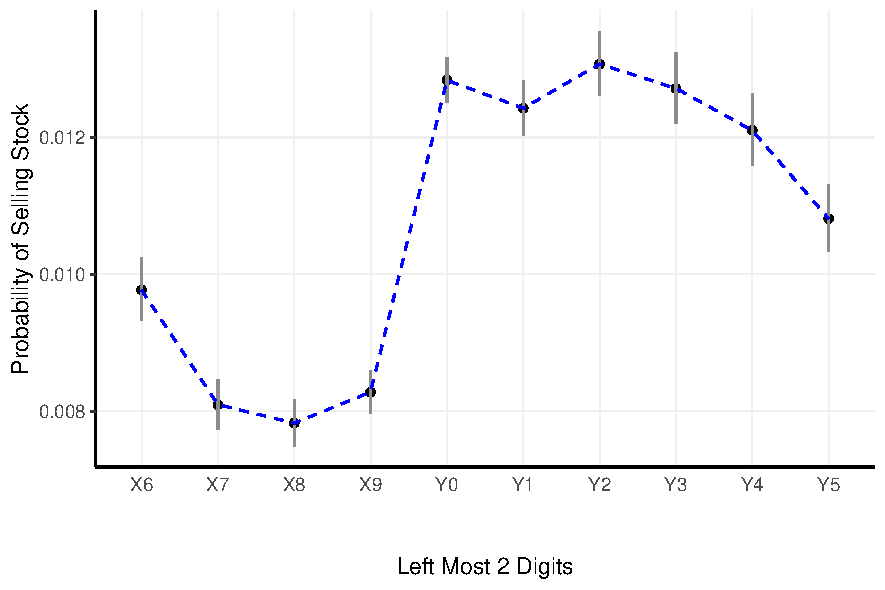
\includegraphics[width=0.45\textwidth]{figures/EndDayLeft2increase_probCI_quarter.pdf}
		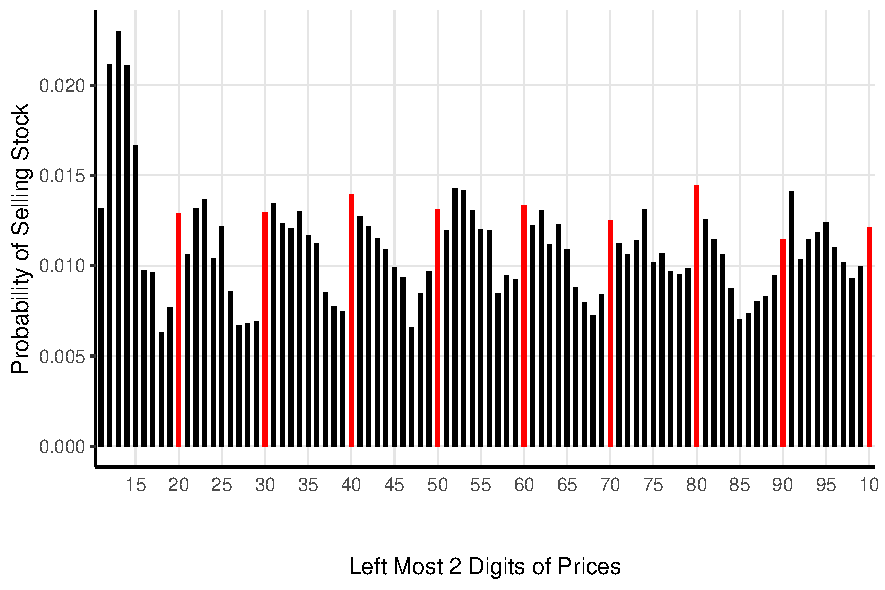
\includegraphics[width=0.45\textwidth]{figures/EndDay2left_increase_quarter.pdf}	
	}
	\subfigure[Price Decreasing]{
		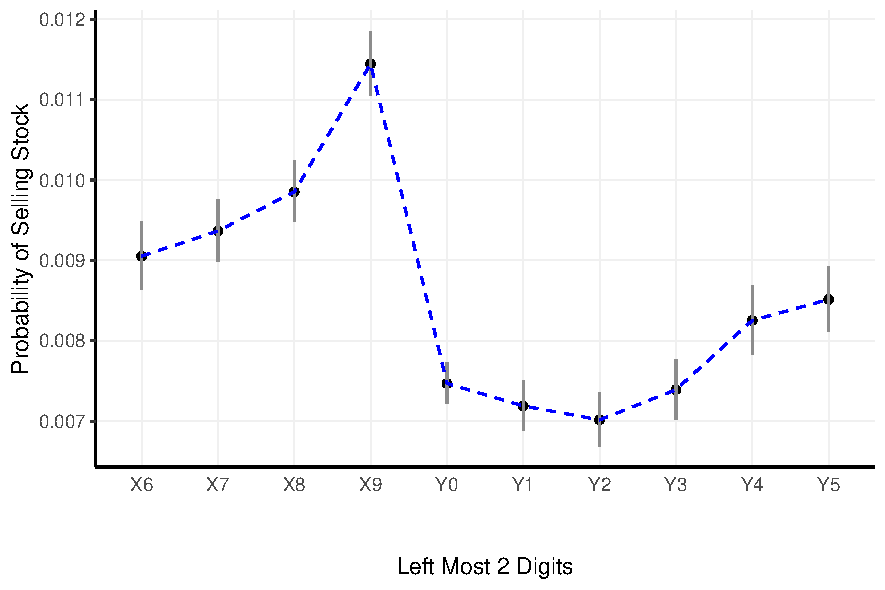
\includegraphics[width=0.45\textwidth]{figures/EndDayLeft2decrease_probCI_quarter.pdf}
		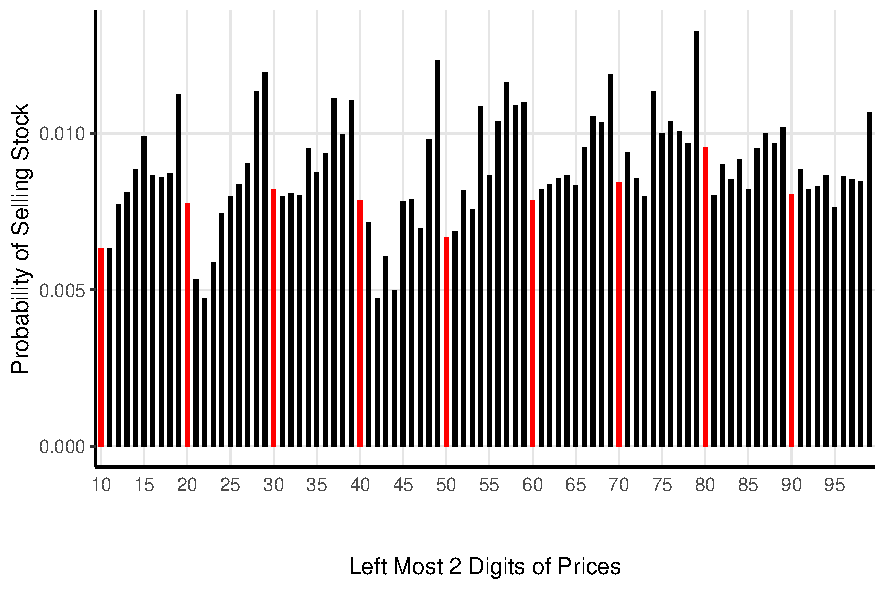
\includegraphics[width=0.45\textwidth]{figures/EndDay2left_decrease_quarter.pdf}	
	}
	\fignote{£$Y$ in the X-axes is equivalent to £$X+1$ (e.g., £X9 could include £0.19, £1.9, £19, etc., while £Y0 could include £0.20, £2.0, £20, etc.).}
\end{figure}

\begin{figure}[hbt!]
	\caption{Leftmost Stock Price Digit and Probability of Sale, Quarterly Sample \\ \textcolor{blue}{Sell-Price, Login Days}}%
	\label{fig:left_digit_sell_main_sell}%
	\centering%	
	\bigskip %liquidLeft2increase_probCI_quarter
	\subfigure[Price Increasing]{
		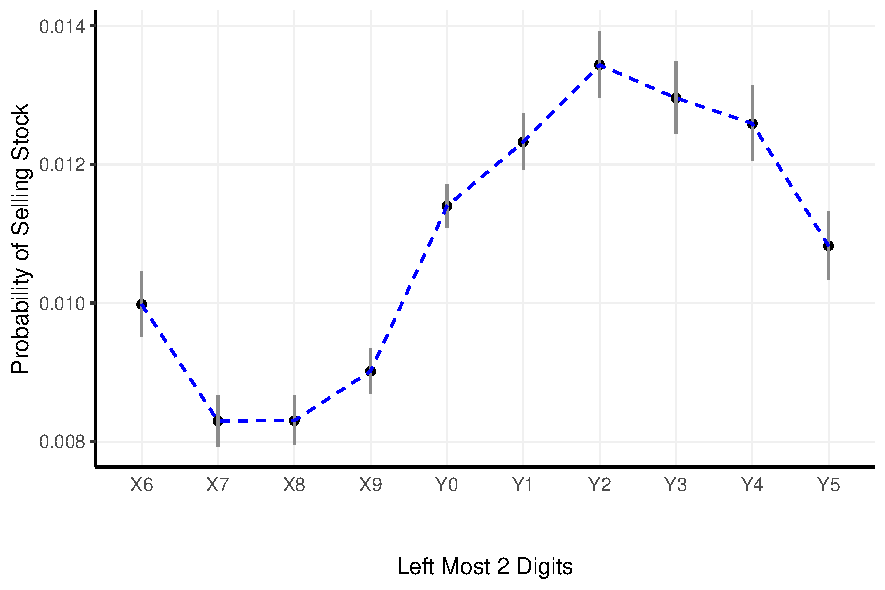
\includegraphics[width=0.45\textwidth]{figures/Left2increase_probCI_quarter.pdf}
		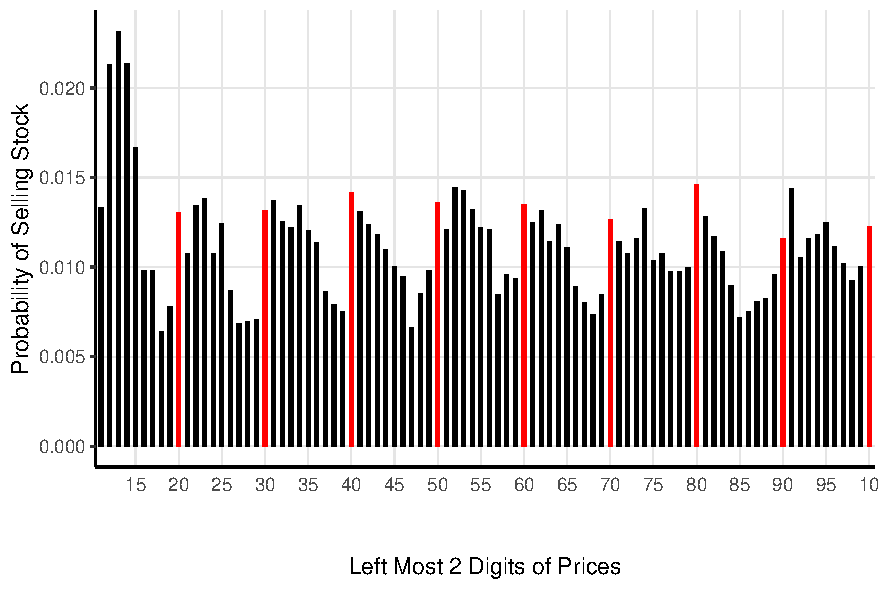
\includegraphics[width=0.45\textwidth]{figures/2left_increase_quarter.pdf}	
	}
	\subfigure[Price Decreasing]{
		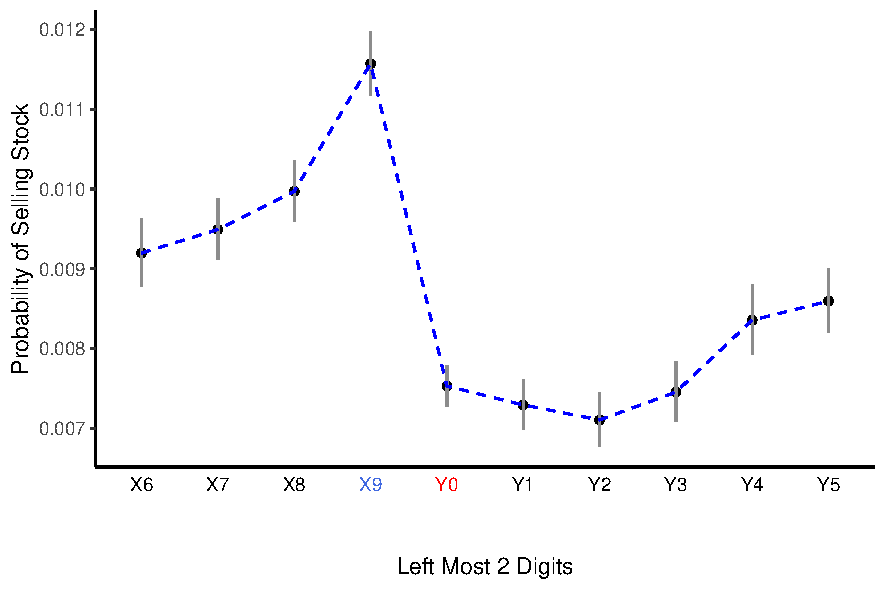
\includegraphics[width=0.45\textwidth]{figures/Left2decrease_probCI_quarter.pdf}
		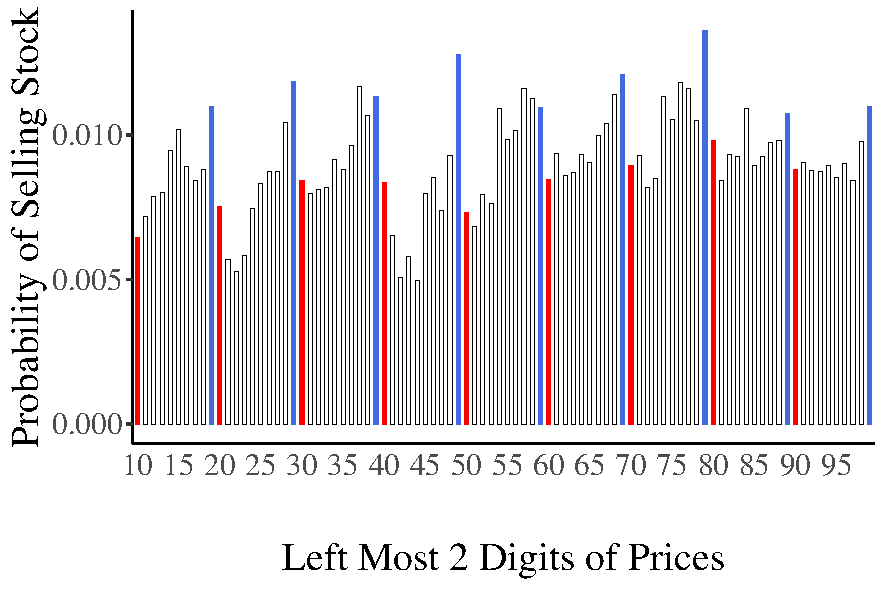
\includegraphics[width=0.45\textwidth]{figures/2left_decrease_quarter.pdf}	
	}
	\fignote{£$Y$ in the X-axes is equivalent to £$X+1$ (e.g., £X9 could include £0.19, £1.9, £19, etc., while £Y0 could include £0.20, £2.0, £20, etc.).}
\end{figure}


\begin{figure}[hbt!]
	\caption{Leftmost Stock Price Digit and Probability of Sale, Quarterly Sample \\ \textcolor{blue}{Sell-Price-No-Login-Yesterday, Login-Days}}%
	\label{fig:left_digit_sell_main_no_yest}%
	\centering%	
	\bigskip %liquidLeft2increase_probCI_quarter
	\subfigure[Price Increasing]{
		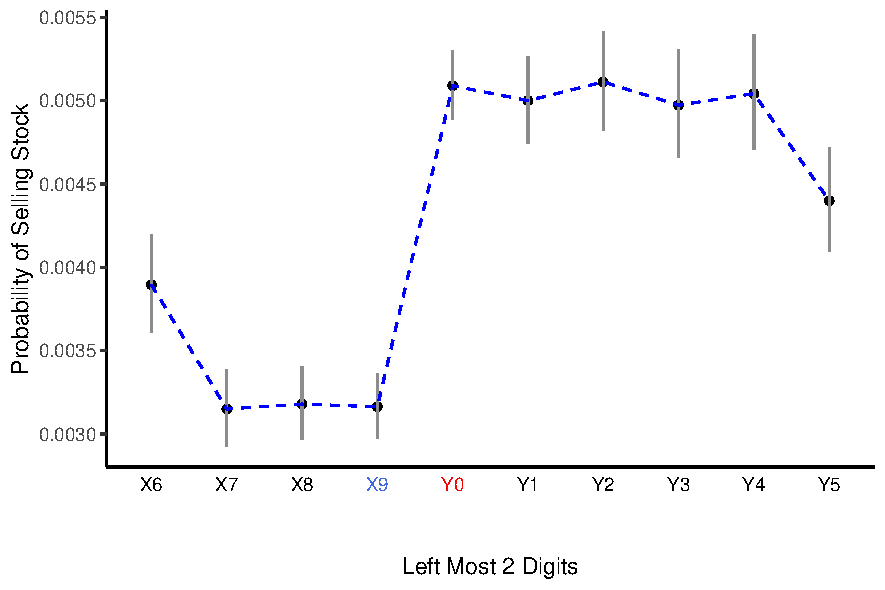
\includegraphics[width=0.45\textwidth]{figures/no_yest_loginLeft2increase_probCI_quarter.pdf}
		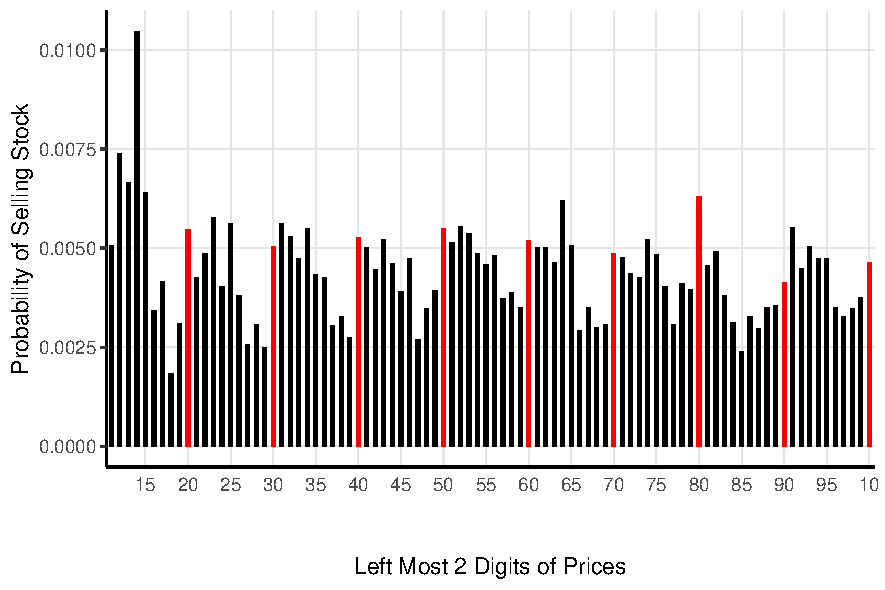
\includegraphics[width=0.45\textwidth]{figures/no_yest_login2left_increase_quarter.pdf}	
	}
	\subfigure[Price Decreasing]{
		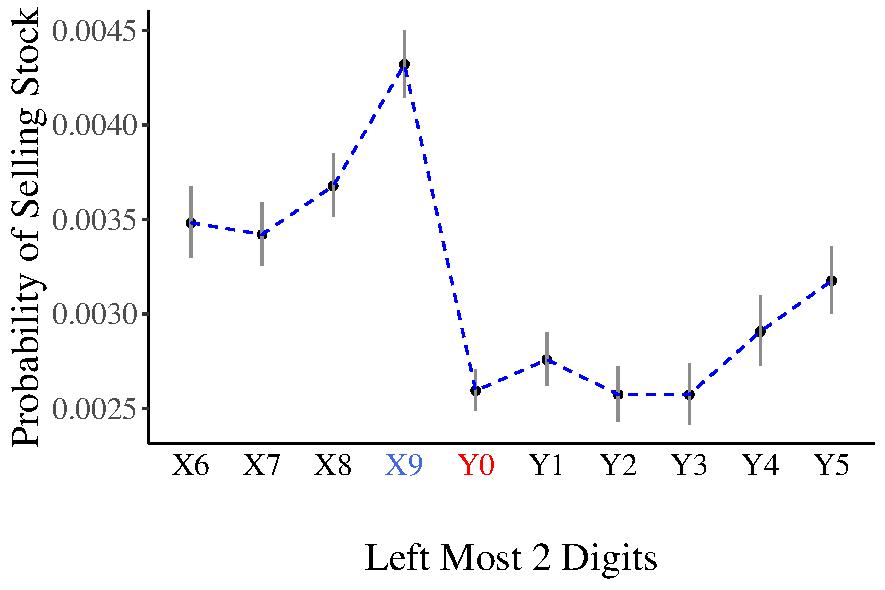
\includegraphics[width=0.45\textwidth]{figures/no_yest_loginLeft2decrease_probCI_quarter.pdf}
		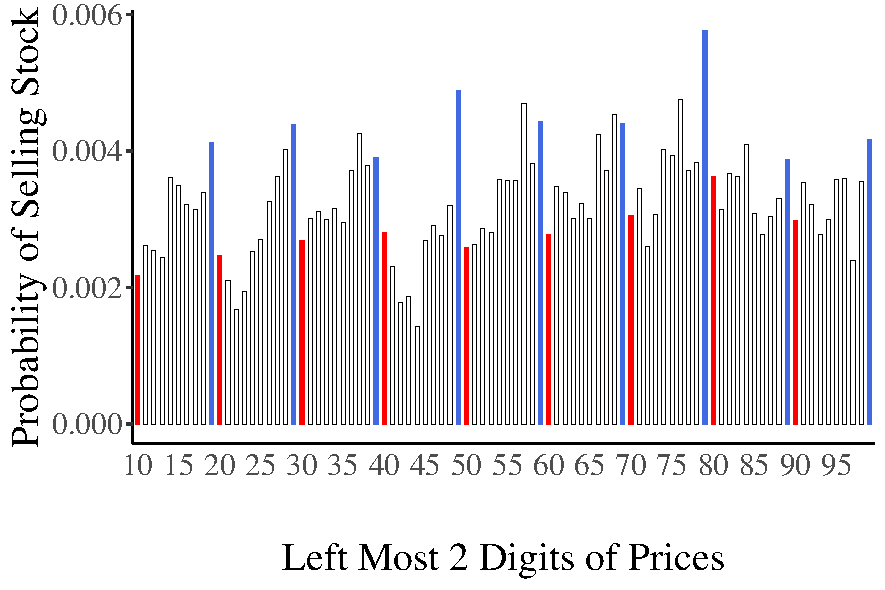
\includegraphics[width=0.45\textwidth]{figures/no_yest_login2left_decrease_quarter.pdf}	
	}
	\fignote{£$Y$ in the X-axes is equivalent to £$X+1$ (e.g., £X9 could include £0.19, £1.9, £19, etc., while £Y0 could include £0.20, £2.0, £20, etc.).}
\end{figure}
\begin{figure}[hbt!]
	\caption{Leftmost Stock Price Digit and Probability of Sale, Quarterly Sample \\ \textcolor{blue}{Sell-Price-FTSE100, Login-Days}}%
	\label{fig:left_digit_sell_main_ftse}%
	\centering%	
	\bigskip %liquidLeft2increase_probCI_quarter
	\subfigure[Price Increasing]{
		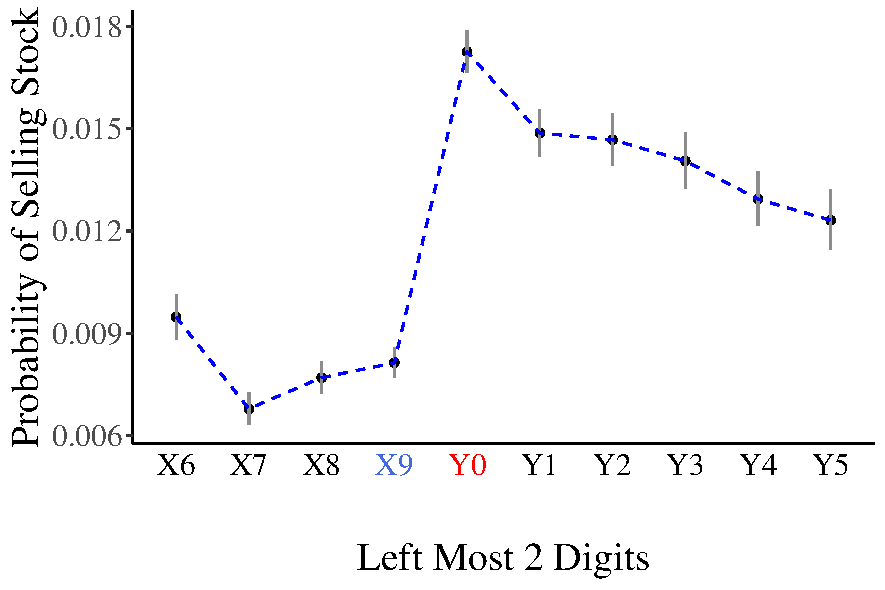
\includegraphics[width=0.45\textwidth]{figures/liquidLeft2increase_probCI_quarter.pdf}
		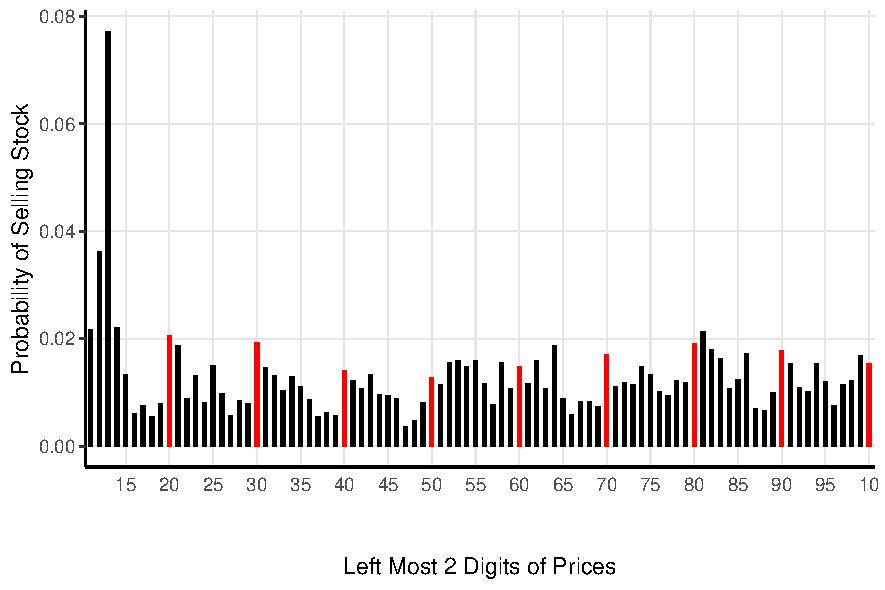
\includegraphics[width=0.45\textwidth]{figures/liquid2left_increase_quarter.pdf}	
	}
	\subfigure[Price Decreasing]{
		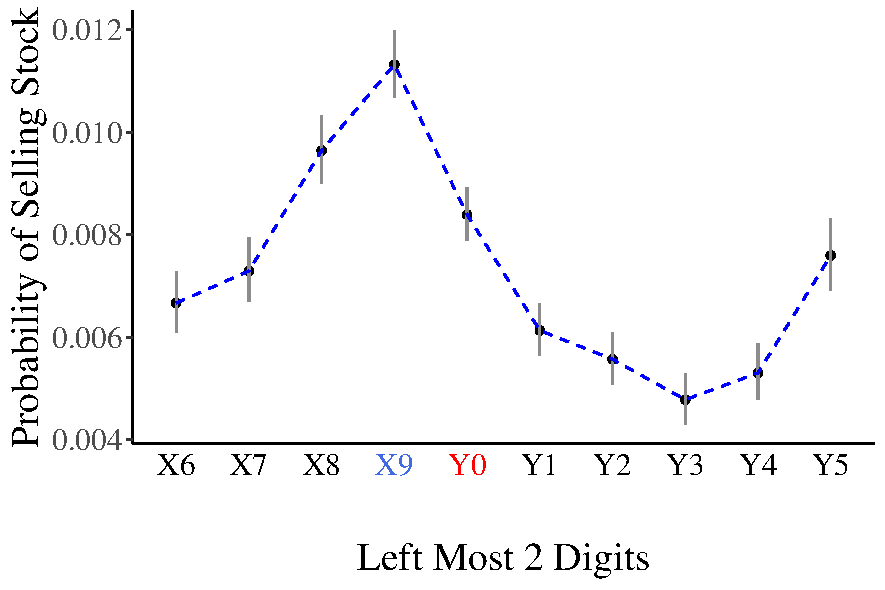
\includegraphics[width=0.45\textwidth]{figures/liquidLeft2decrease_probCI_quarter.pdf}
		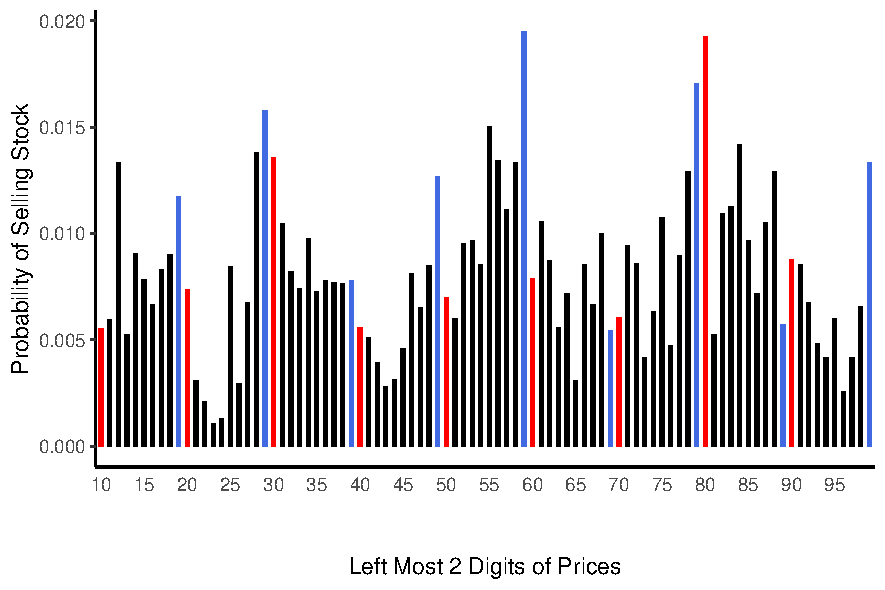
\includegraphics[width=0.45\textwidth]{figures/liquid2left_decrease_quarter.pdf}	
	}
	\fignote{£$Y$ in the X-axes is equivalent to £$X+1$ (e.g., £X9 could include £0.19, £1.9, £19, etc., while £Y0 could include £0.20, £2.0, £20, etc.).}
\end{figure}

\clearpage


%subset of prices
\begin{figure}[hbt!]
	\caption{Leftmost Stock Price Digit and Probability of Sale \\ Prices Increasing Sample by Price Range \\ \textcolor{blue}{Market-Price, Login-Days}}%
	\label{fig:left_digit_sell_increase_mainsss_market}%
	\centering%	
	\bigskip
	\subfigure[Price = \pounds0.11 to \pounds1.01]{
		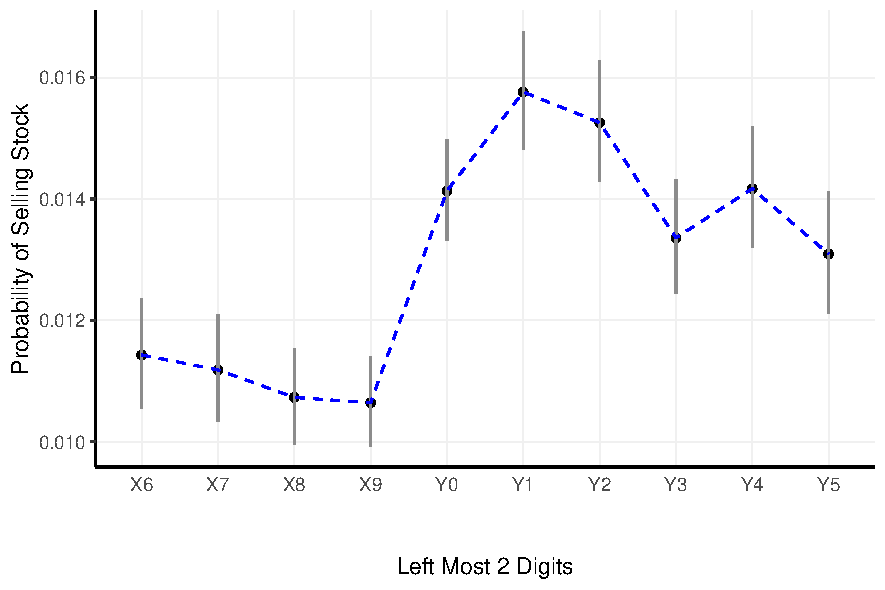
\includegraphics[width=0.45\textwidth]{figures/EndDayLeft2increases_1pbin_CI_quarter.pdf}
		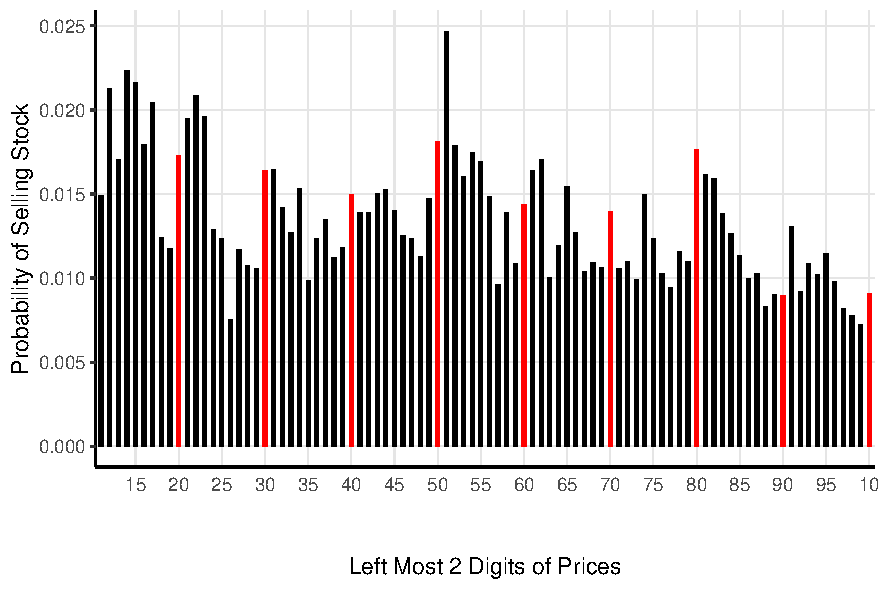
\includegraphics[width=0.45\textwidth]{figures/EndDay2left_increase_bin1p_quarter.pdf}
	}
	\subfigure[Price = \pounds1.01 to \pounds10.1]{
		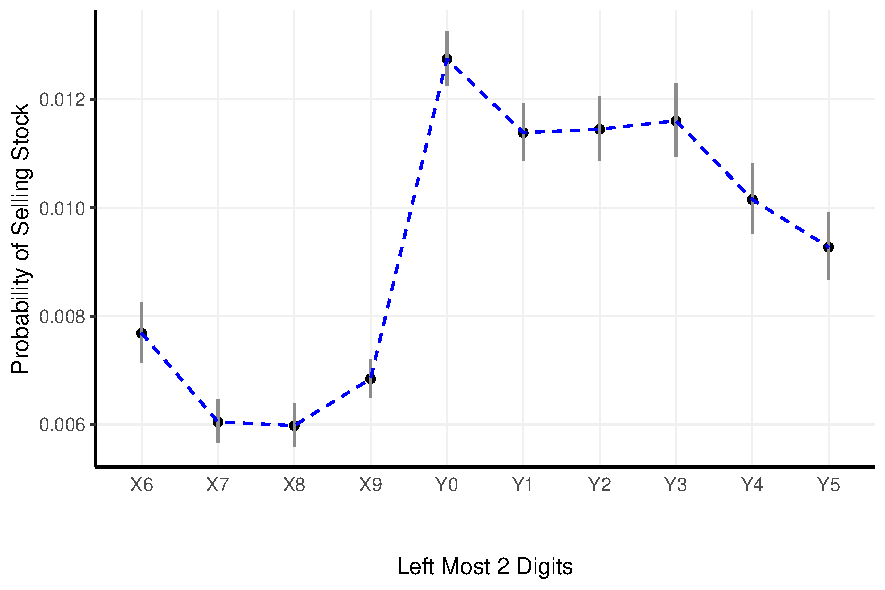
\includegraphics[width=0.45\textwidth]{figures/EndDayLeft2increases_10pbin_CI_quarter.pdf}
		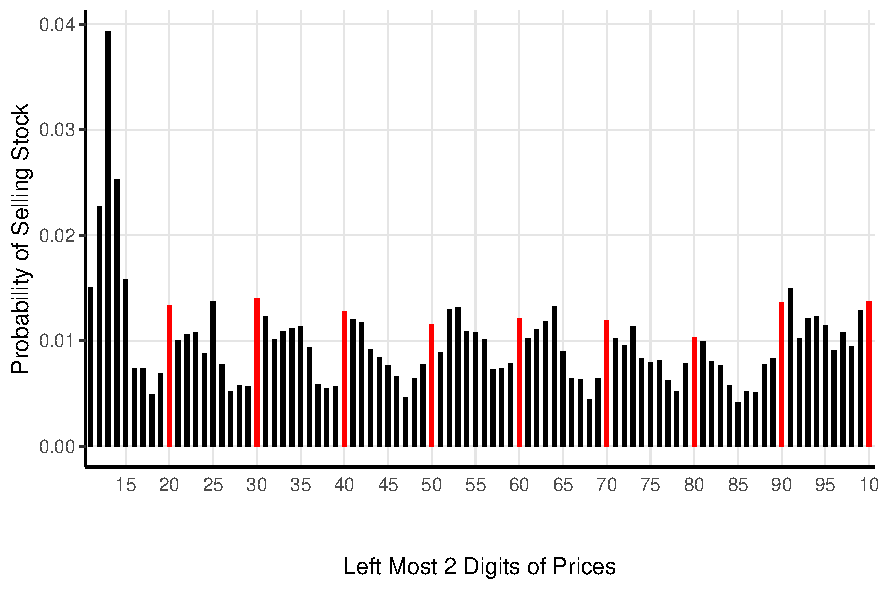
\includegraphics[width=0.45\textwidth]{figures/EndDay2left_increase_bin10p_quarter.pdf}
	}
	\subfigure[Price = \pounds11 to \pounds101]{
		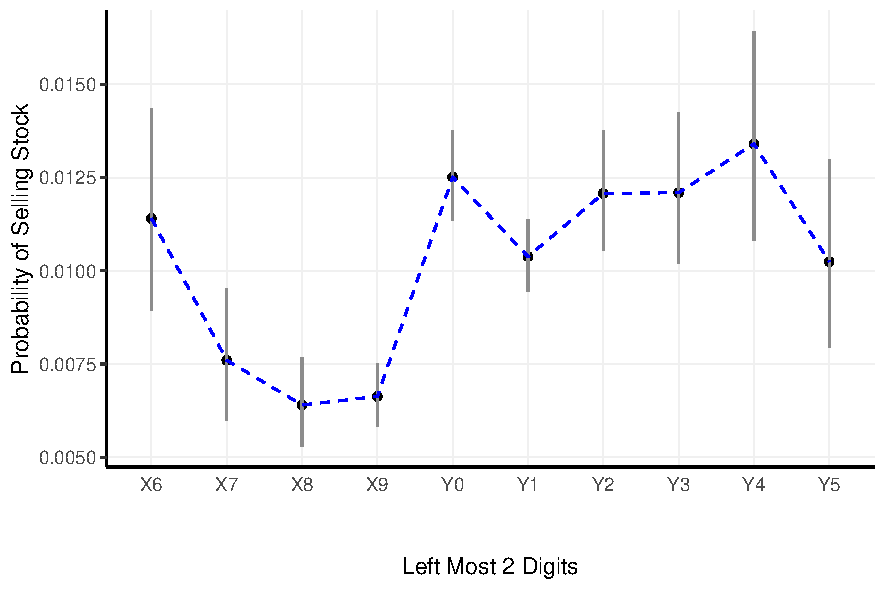
\includegraphics[width=0.45\textwidth]{figures/EndDayLeft2increases_1poundbin_CI_quarter.pdf}
		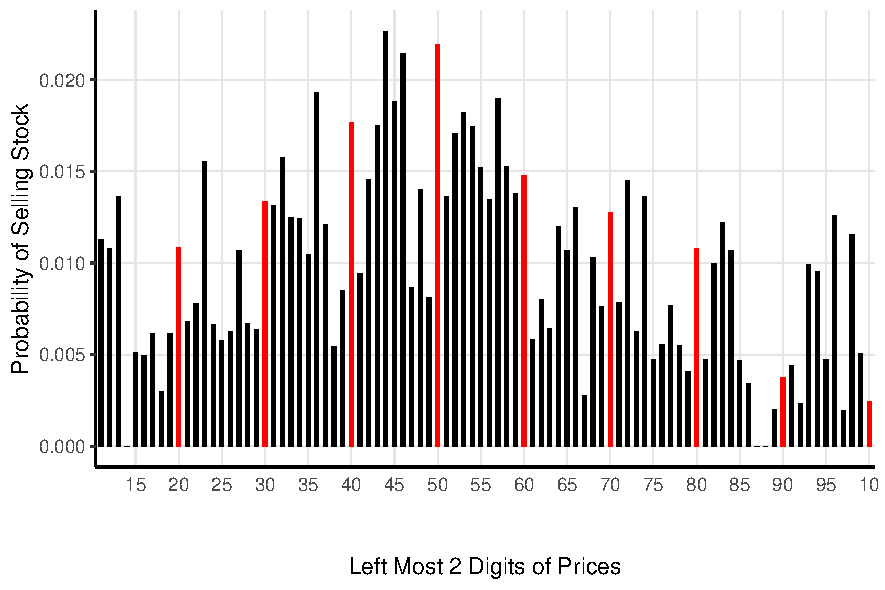
\includegraphics[width=0.45\textwidth]{figures/EndDay2left_increase_bin1pound_quarter.pdf}
	}
	\fignote{£$Y$ in the X-axes is equivalent to £$X+1$ (e.g., £X9 could include £0.19, £1.9, £19, etc., while £Y0 could include £0.20, £2.0, £20, etc.). Panels A, B and C show equal size bins of 1p, 10p and £1, respectively. Panel A corresponds to 25\% of the observations in the prices increasing sample; Panel B, to 55\%; and Panel C, to 8\%.}
\end{figure}

\begin{figure}[hbt!]
	\caption{Leftmost Stock Price Digit and Probability of Sale \\ Prices Increasing Sample by Price Range \\ \textcolor{blue}{Sell-Price, Login-Days}}%
	\label{fig:left_digit_sell_increase_mainsss_sell}%
	\centering%	
	\bigskip
	\subfigure[Price = \pounds0.11 to \pounds1.01]{
		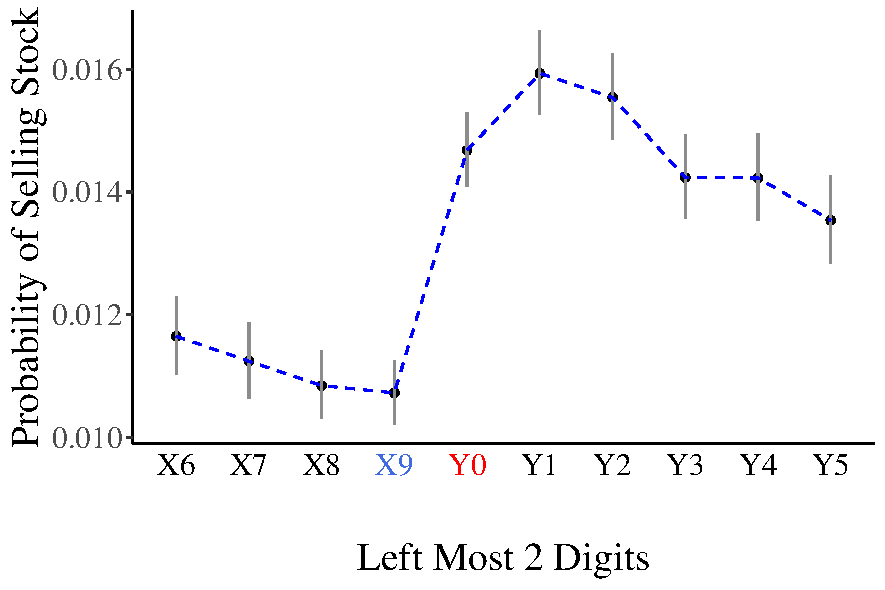
\includegraphics[width=0.45\textwidth]{figures/Left2increases_1pbin_CI_quarter.pdf}
		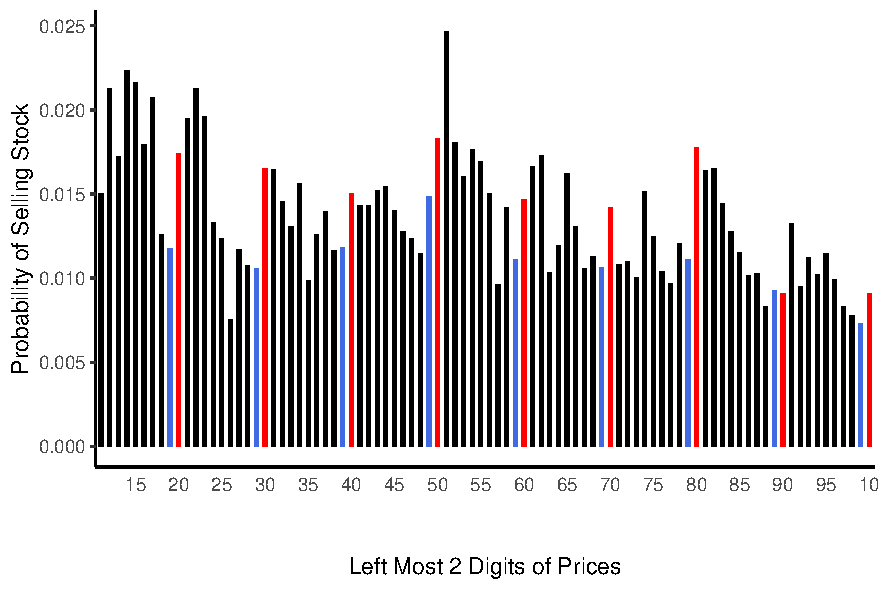
\includegraphics[width=0.45\textwidth]{figures/2left_increase_bin1p_quarter.pdf}
	}
	\subfigure[Price = \pounds1.01 to \pounds10.1]{
		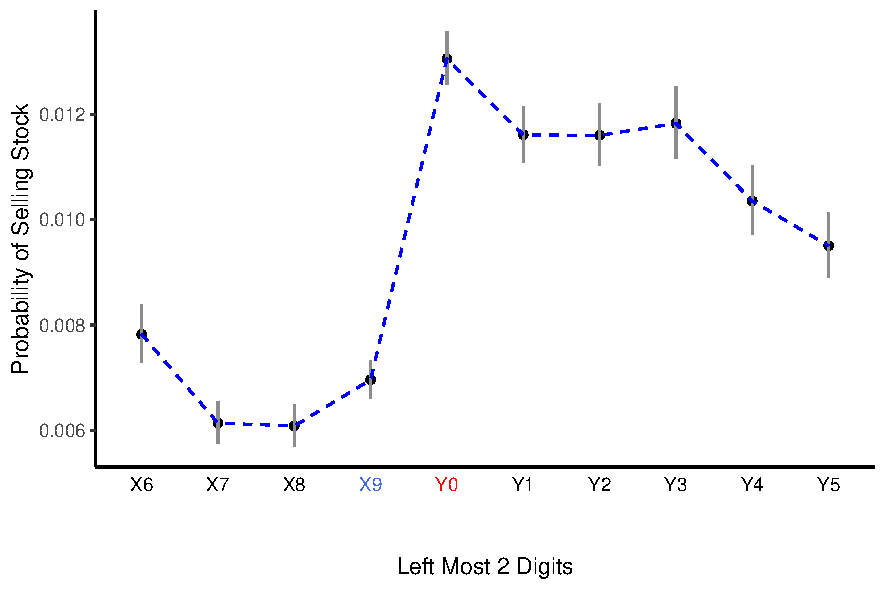
\includegraphics[width=0.45\textwidth]{figures/Left2increases_10pbin_CI_quarter.pdf}
		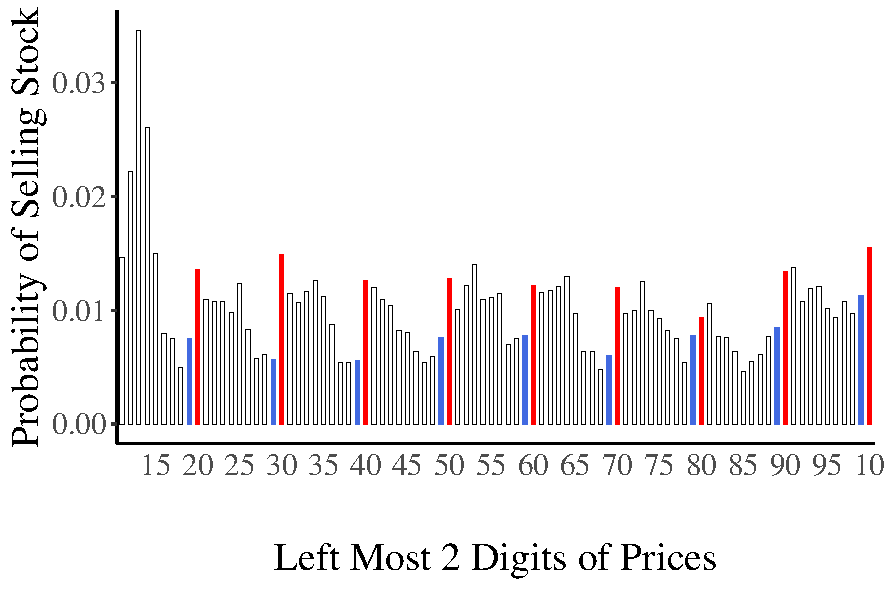
\includegraphics[width=0.45\textwidth]{figures/2left_increase_bin10p_quarter.pdf}
	}
	\subfigure[Price = \pounds11 to \pounds101]{
		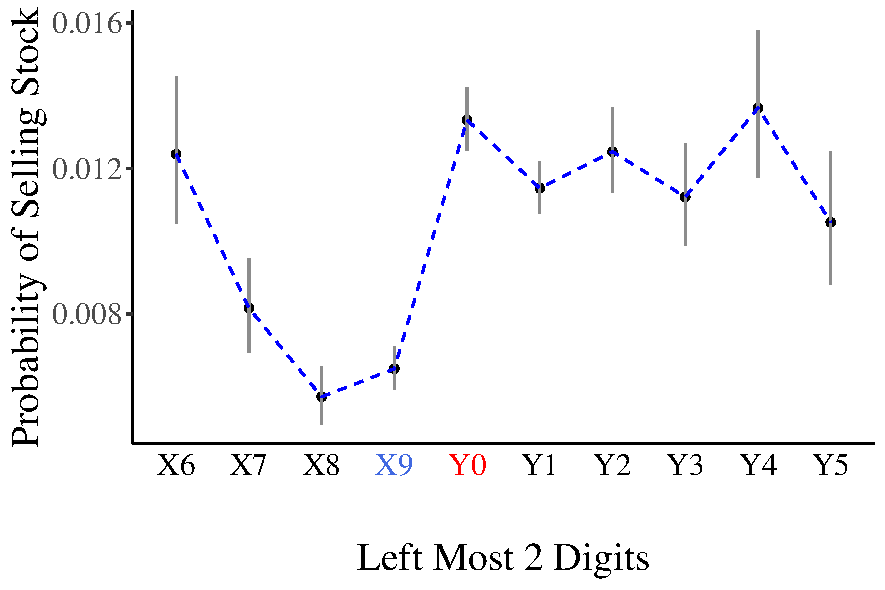
\includegraphics[width=0.45\textwidth]{figures/Left2increases_1poundbin_CI_quarter.pdf}
		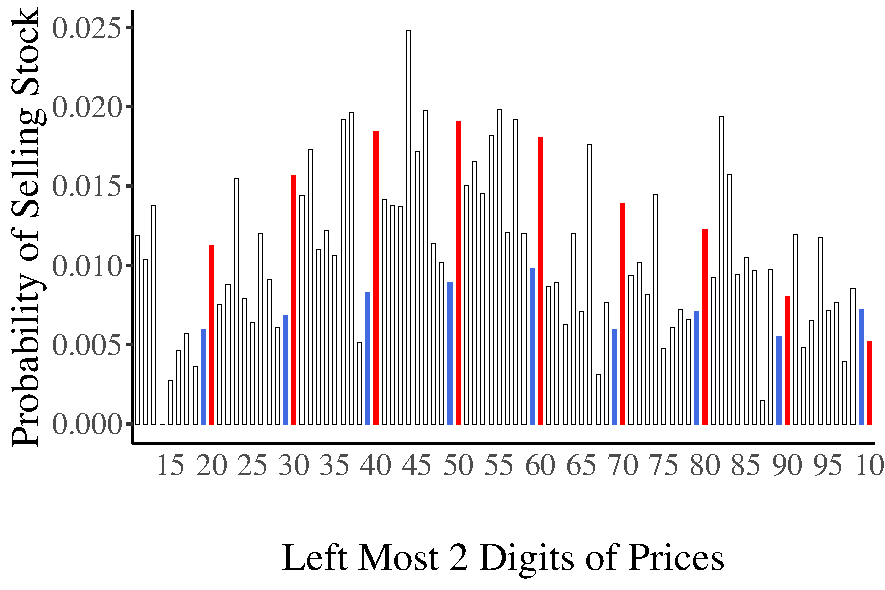
\includegraphics[width=0.45\textwidth]{figures/2left_increase_bin1pound_quarter.pdf}
	}
	\fignote{£$Y$ in the X-axes is equivalent to £$X+1$ (e.g., £X9 could include £0.19, £1.9, £19, etc., while £Y0 could include £0.20, £2.0, £20, etc.). Panels A, B and C show equal size bins of 1p, 10p and £1, respectively. Panel A corresponds to 25\% of the observations in the prices increasing sample; Panel B, to 55\%; and Panel C, to 8\%.}
\end{figure}

\begin{figure}[hbt!]
	\caption{Leftmost Stock Price Digit and Probability of Sale \\ Prices Increasing Sample by Price Range \\ \textcolor{blue}{Sell-Price-No-Login-Yesterday, Login-Days}}%
	\label{fig:left_digit_sell_increase_mainsss_no_yest}%
	\centering%	
	\bigskip
	\subfigure[Price = \pounds0.11 to \pounds1.01]{
		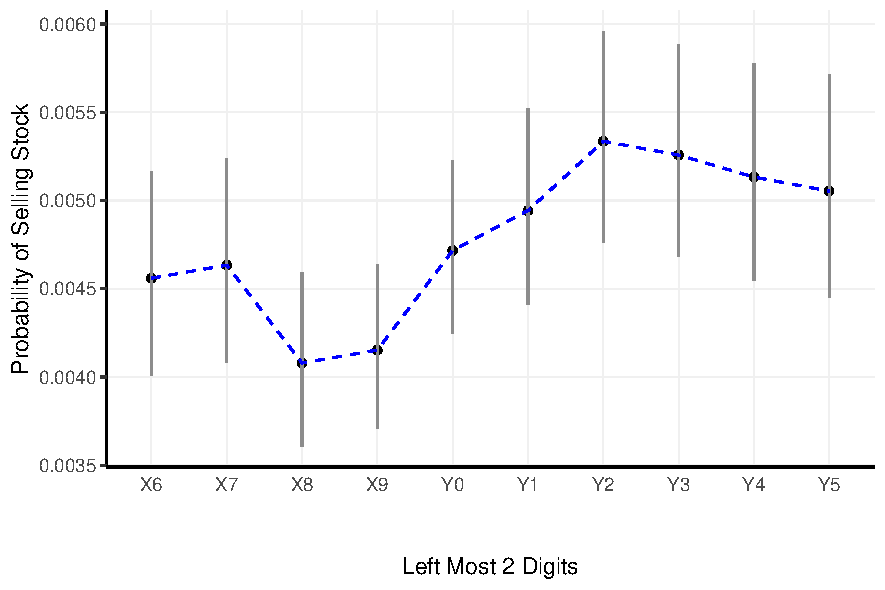
\includegraphics[width=0.45\textwidth]{figures/no_yest_loginLeft2increases_1pbin_CI_quarter.pdf}
		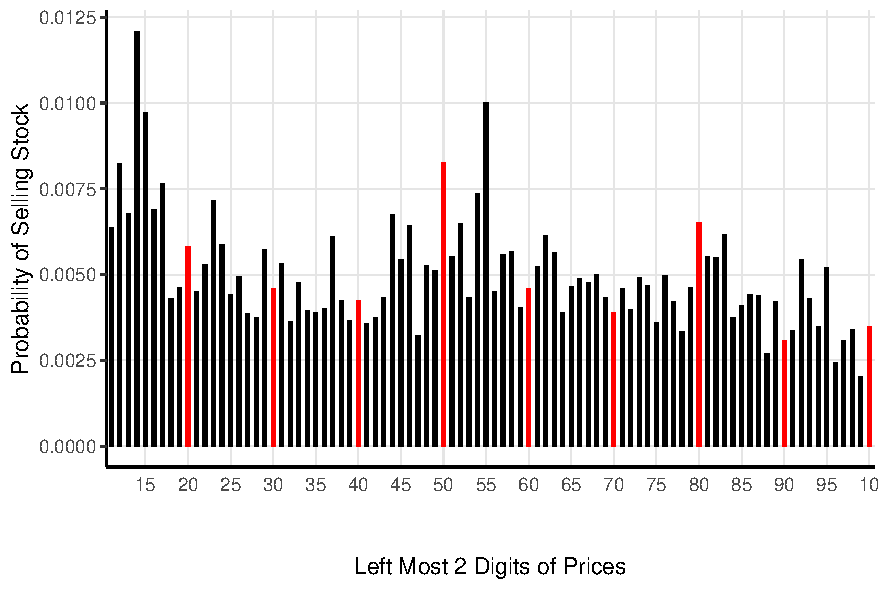
\includegraphics[width=0.45\textwidth]{figures/no_yest_login2left_increase_bin1p_quarter.pdf}
	}
	\subfigure[Price = \pounds1.01 to \pounds10.1]{
		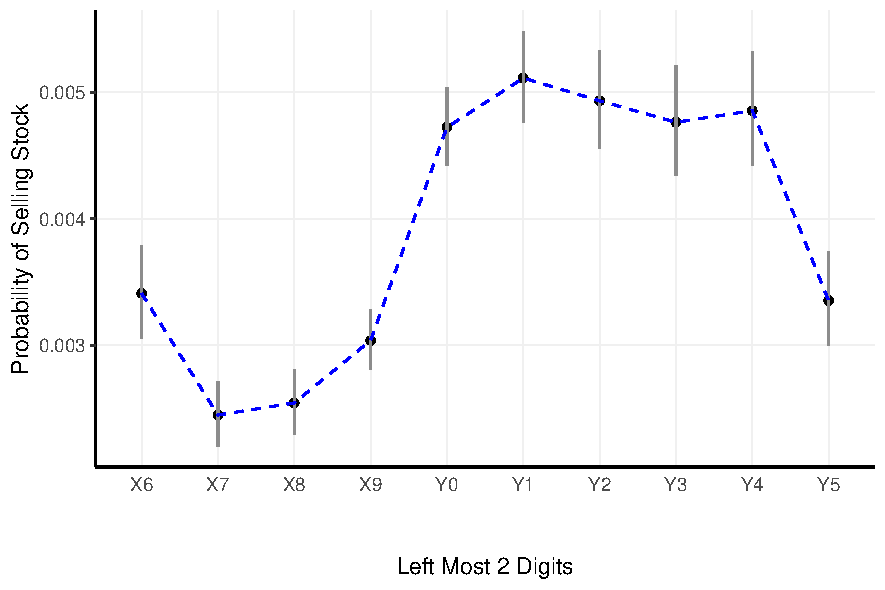
\includegraphics[width=0.45\textwidth]{figures/no_yest_loginLeft2increases_10pbin_CI_quarter.pdf}
		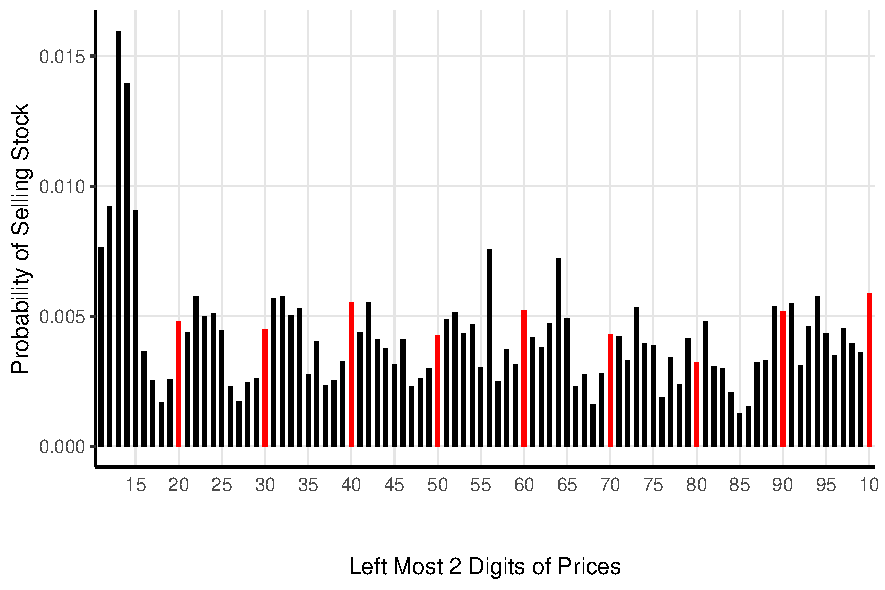
\includegraphics[width=0.45\textwidth]{figures/no_yest_login2left_increase_bin10p_quarter.pdf}
	}
	\subfigure[Price = \pounds11 to \pounds101]{
		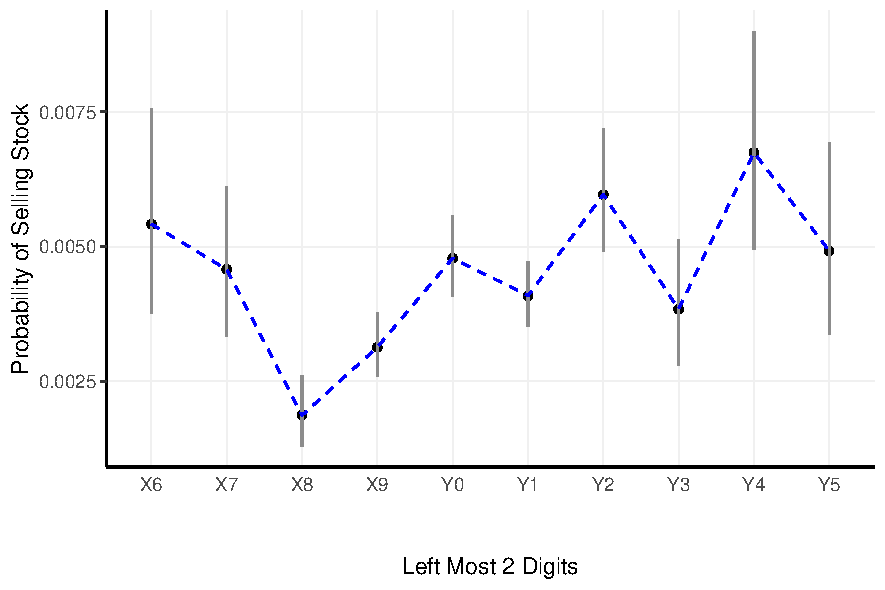
\includegraphics[width=0.45\textwidth]{figures/no_yest_loginLeft2increases_1poundbin_CI_quarter.pdf}
		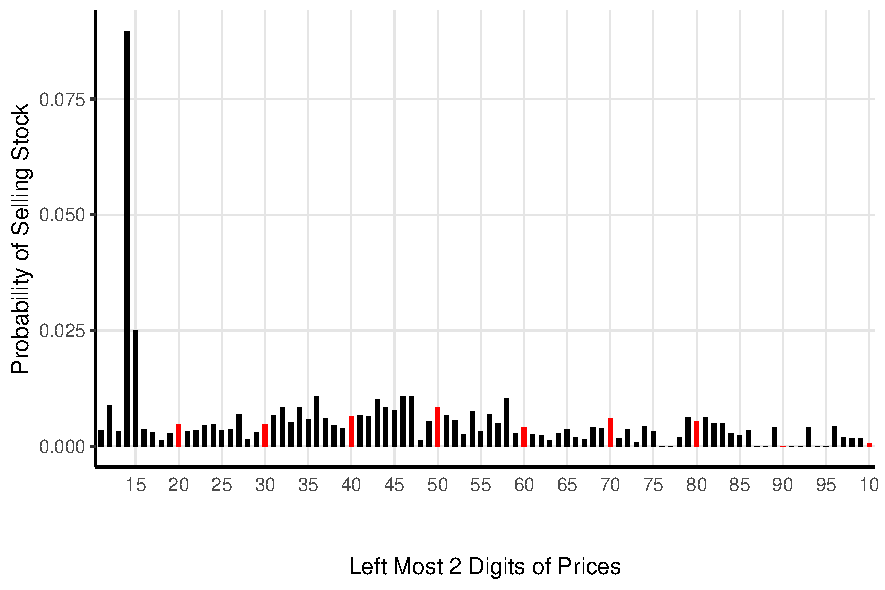
\includegraphics[width=0.45\textwidth]{figures/no_yest_login2left_increase_bin1pound_quarter.pdf}
	}
	\fignote{£$Y$ in the X-axes is equivalent to £$X+1$ (e.g., £X9 could include £0.19, £1.9, £19, etc., while £Y0 could include £0.20, £2.0, £20, etc.). Panels A, B and C show equal size bins of 1p, 10p and £1, respectively. Panel A corresponds to 25\% of the observations in the prices increasing sample; Panel B, to 55\%; and Panel C, to 8\%.}
\end{figure}

\begin{figure}[hbt!]
	\caption{Leftmost Stock Price Digit and Probability of Sale \\ Prices Increasing Sample by Price Range \\ \textcolor{blue}{Sell-Price-FTSE100, Login-Days}}%
	\label{fig:left_digit_sell_increase_mainsss_ftse}%
	\centering%	
	\bigskip
	\subfigure[Price = \pounds0.11 to \pounds1.01]{
		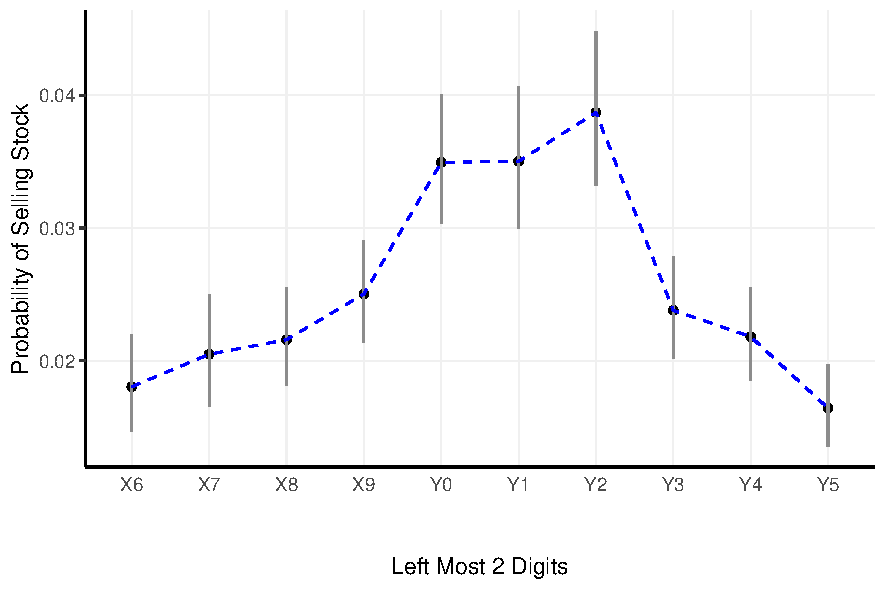
\includegraphics[width=0.45\textwidth]{figures/liquidLeft2increases_1pbin_CI_quarter.pdf}
		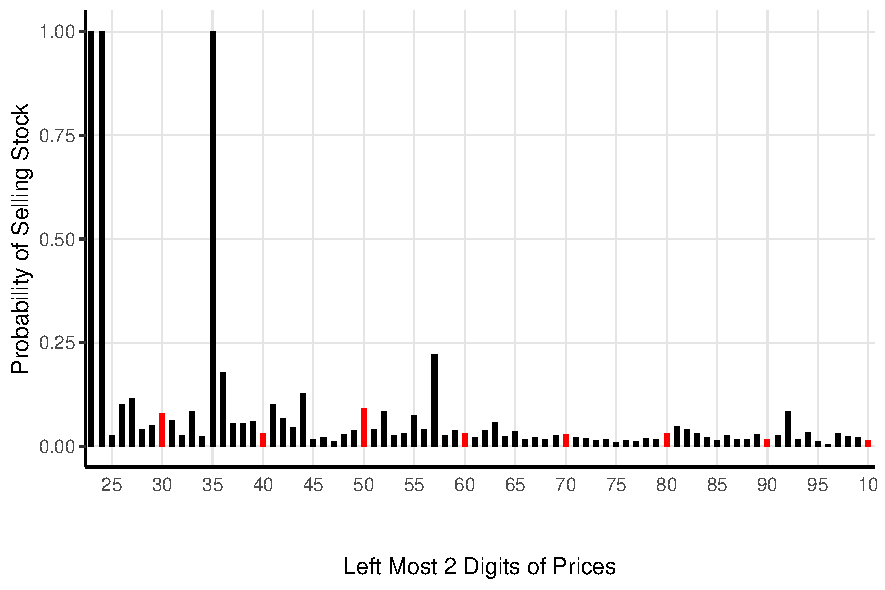
\includegraphics[width=0.45\textwidth]{figures/liquid2left_increase_bin1p_quarter.pdf}
	}
	\subfigure[Price = \pounds1.01 to \pounds10.1]{
		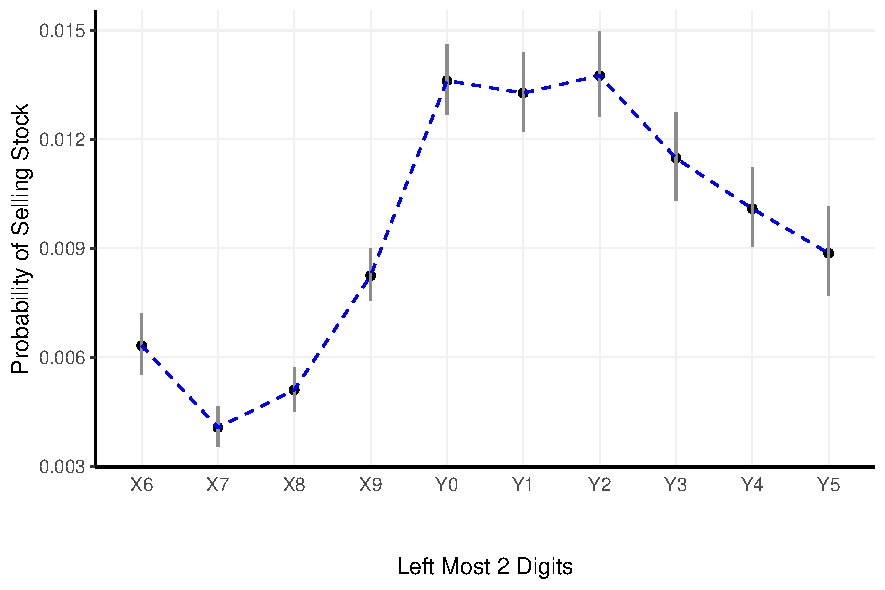
\includegraphics[width=0.45\textwidth]{figures/liquidLeft2increases_10pbin_CI_quarter.pdf}
		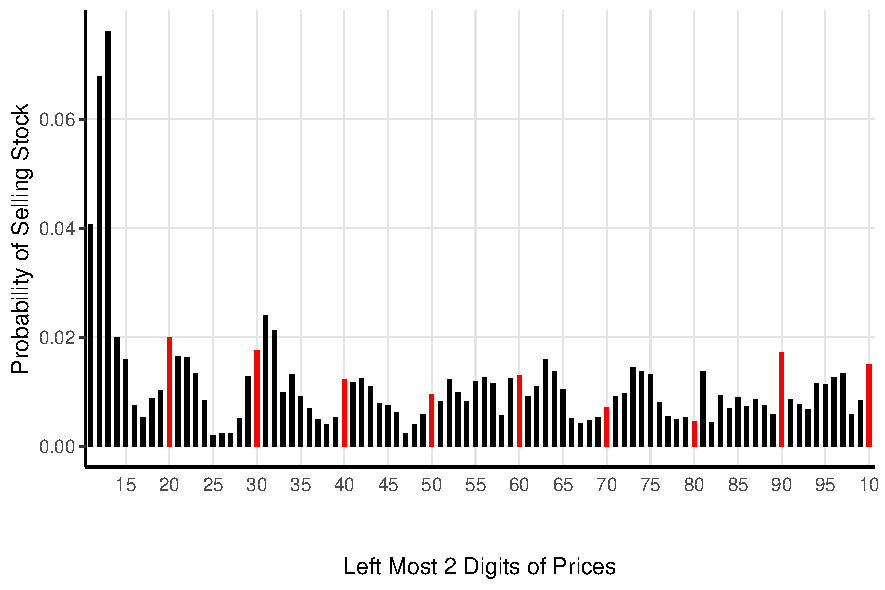
\includegraphics[width=0.45\textwidth]{figures/liquid2left_increase_bin10p_quarter.pdf}
	}
	\subfigure[Price = \pounds11 to \pounds101]{
		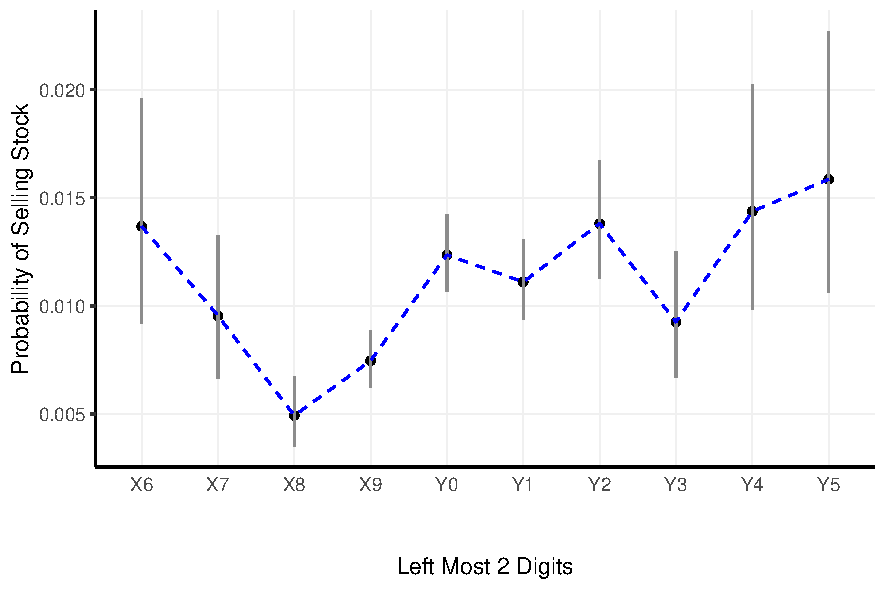
\includegraphics[width=0.45\textwidth]{figures/liquidLeft2increases_1poundbin_CI_quarter.pdf}
		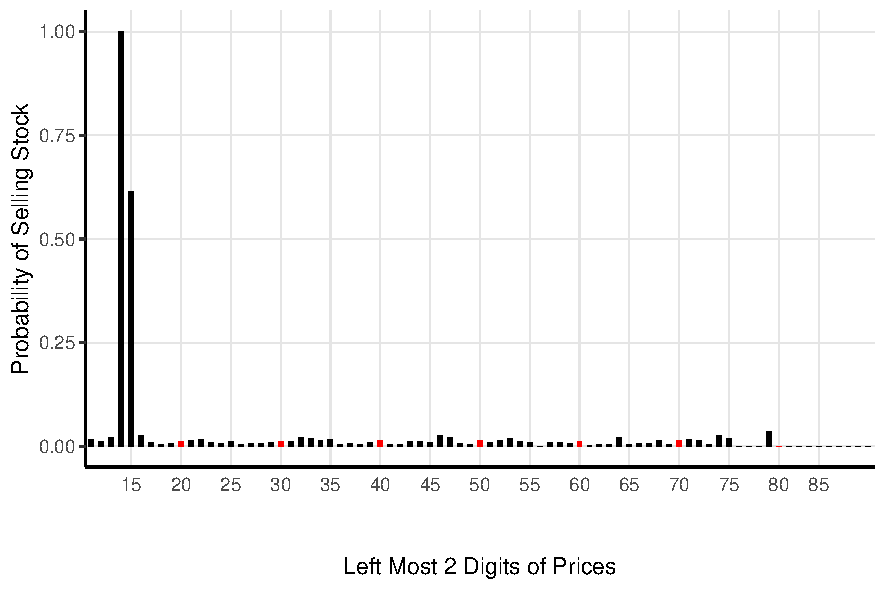
\includegraphics[width=0.45\textwidth]{figures/liquid2left_increase_bin1pound_quarter.pdf}
	}
	\fignote{£$Y$ in the X-axes is equivalent to £$X+1$ (e.g., £X9 could include £0.19, £1.9, £19, etc., while £Y0 could include £0.20, £2.0, £20, etc.). Panels A, B and C show equal size bins of 1p, 10p and £1, respectively. Panel A corresponds to 25\% of the observations in the prices increasing sample; Panel B, to 55\%; and Panel C, to 8\%.}
\end{figure}





\clearpage
\begin{figure}[hbt!]
	\caption{Leftmost Stock Price Digit and Probability of Sale \\ Prices Decreasing Sample by Price Range \\ \textcolor{blue}{Market-Price, Login-Days}}%
	\label{fig:left_digit_sell_decrease_mainsss_market}%
	\centering%	
	\bigskip
	\subfigure[Price = \pounds0.10 to \pounds1.00]{
		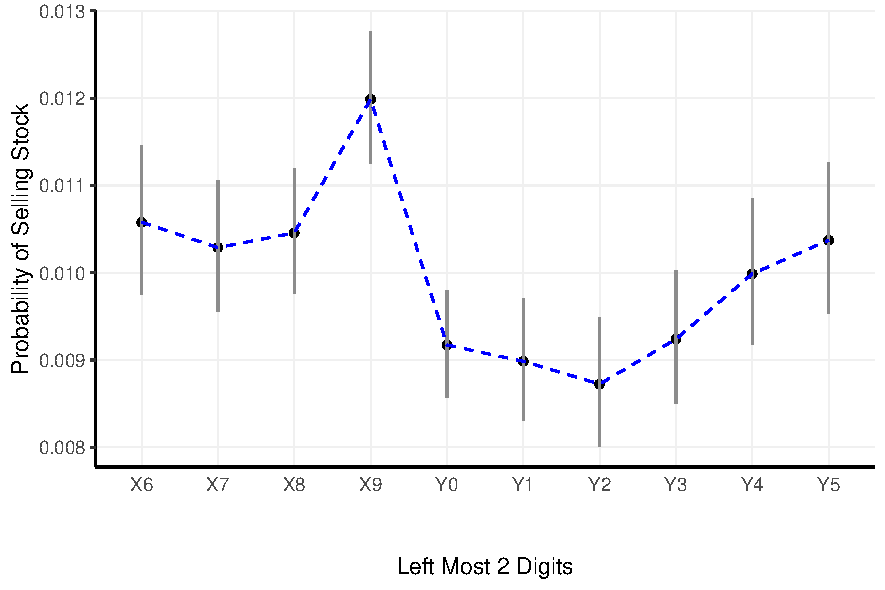
\includegraphics[width=0.45\textwidth]{figures/EndDayLeft2decreases_1pbin_CI_quarter.pdf}
		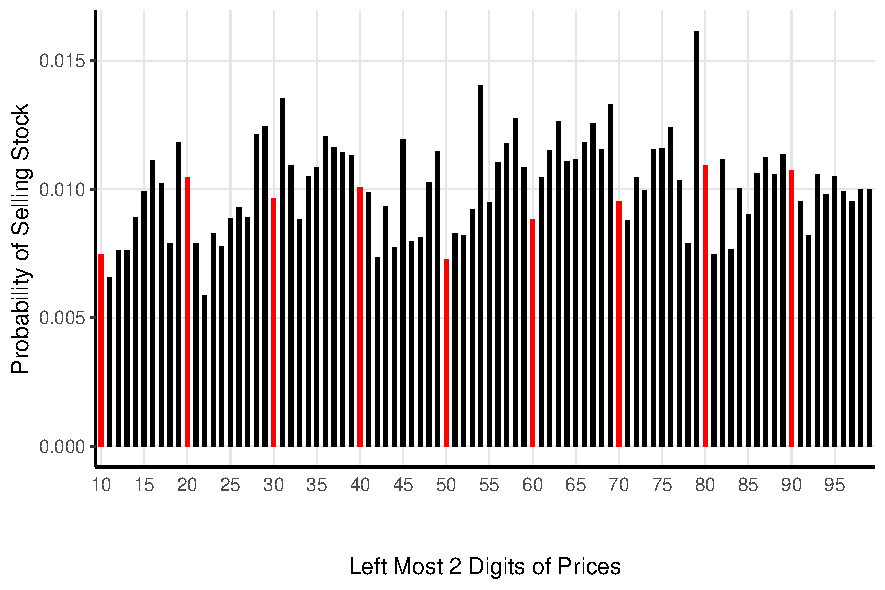
\includegraphics[width=0.45\textwidth]{figures/EndDay2left_decrease_bin1p_quarter.pdf}
	}
	\subfigure[Price = \pounds1.00 to \pounds10.0]{
		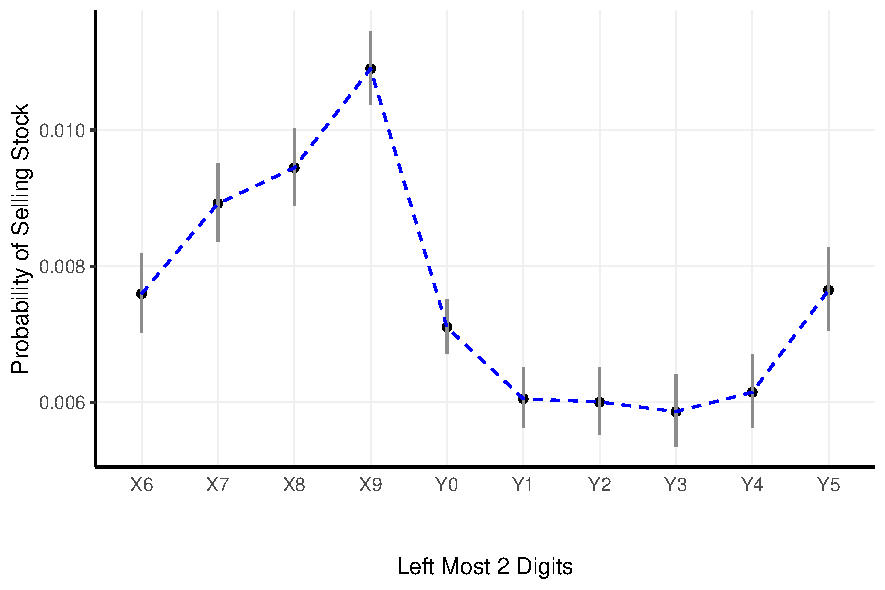
\includegraphics[width=0.45\textwidth]{figures/EndDayLeft2decreases_10pbin_CI_quarter.pdf}
		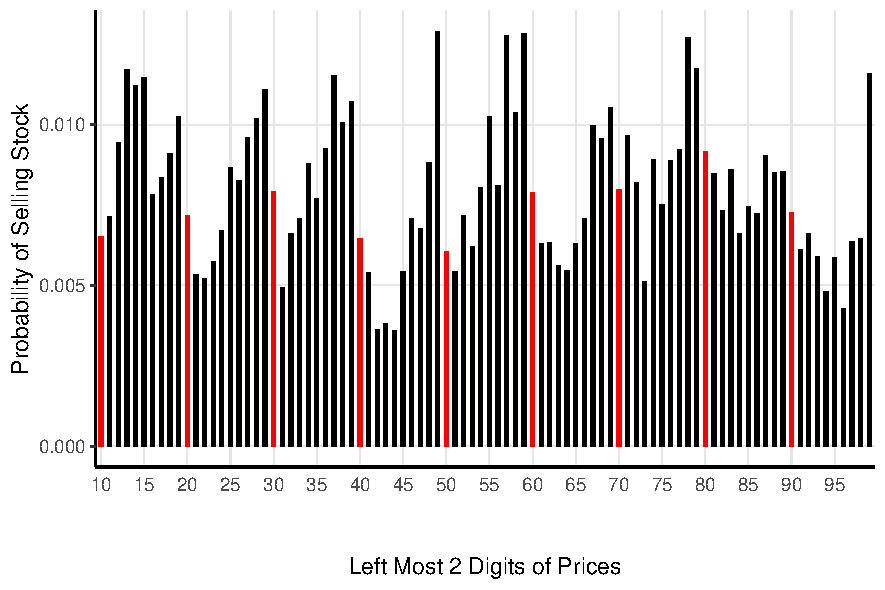
\includegraphics[width=0.45\textwidth]{figures/EndDay2left_decrease_bin10p_quarter.pdf}
	}
	\subfigure[Price = \pounds10 to \pounds100]{
		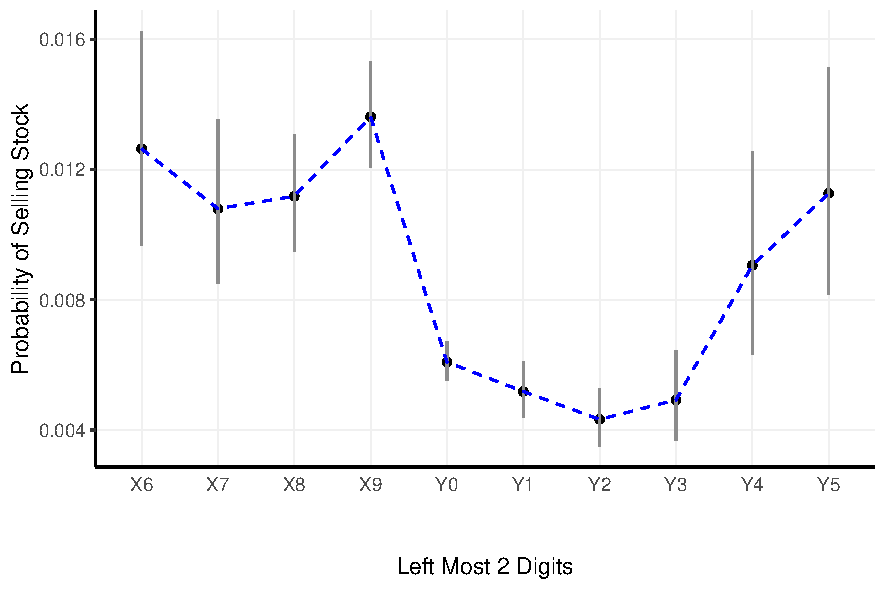
\includegraphics[width=0.45\textwidth]{figures/EndDayLeft2decreases_1poundbin_CI_quarter.pdf}
		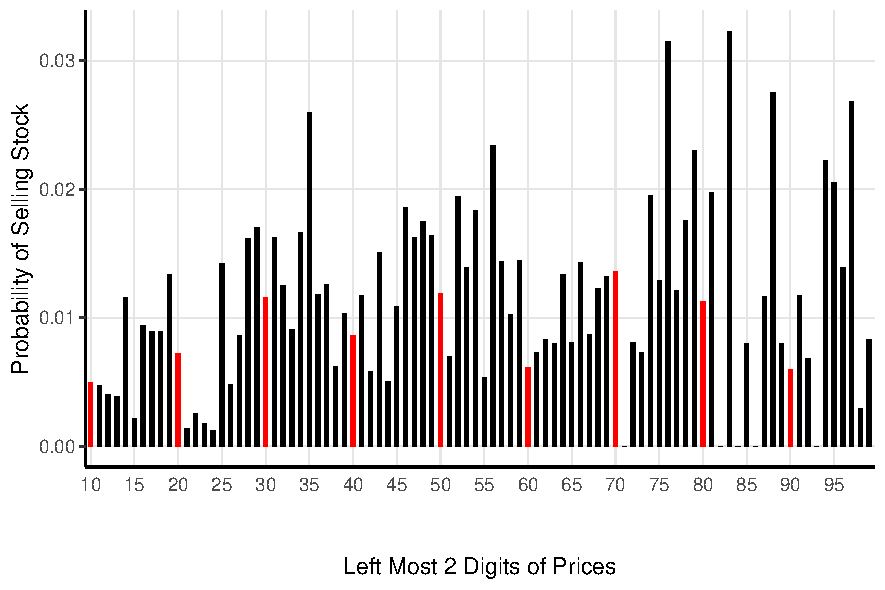
\includegraphics[width=0.45\textwidth]{figures/EndDay2left_decrease_bin1pound_quarter.pdf}
	}
	\fignote{£$Y$ in the X-axes is equivalent to £$X+1$ (e.g., £X9 could include £0.19, £1.9, £19, etc., while £Y0 could include £0.20, £2.0, £20, etc.). Panels A, B and C show equal size bins of 1p, 10p and £1, respectively. Panel A corresponds to 27\% of the observations in the prices decreasing sample; Panel B, to 43\%; and Panel C, to 7\%.}
\end{figure}


\clearpage
\begin{figure}[hbt!]
	\caption{Leftmost Stock Price Digit and Probability of Sale \\ Prices Decreasing Sample by Price Range \\ \textcolor{blue}{Sell-Price, Login-Days}}%
	\label{fig:left_digit_sell_decrease_mainsss_sell}%
	\centering%	
	\bigskip
	\subfigure[Price = \pounds0.10 to \pounds1.00]{
		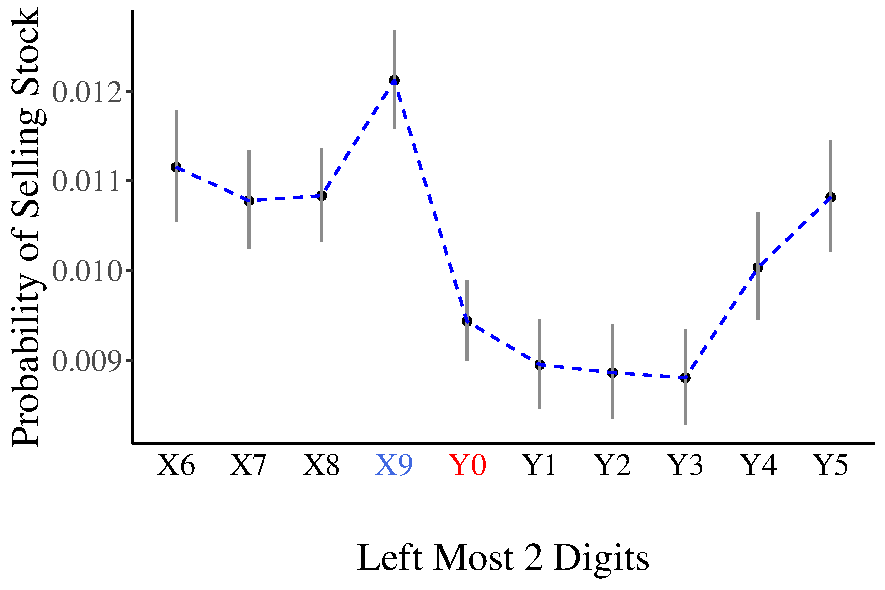
\includegraphics[width=0.45\textwidth]{figures/Left2decreases_1pbin_CI_quarter.pdf}
		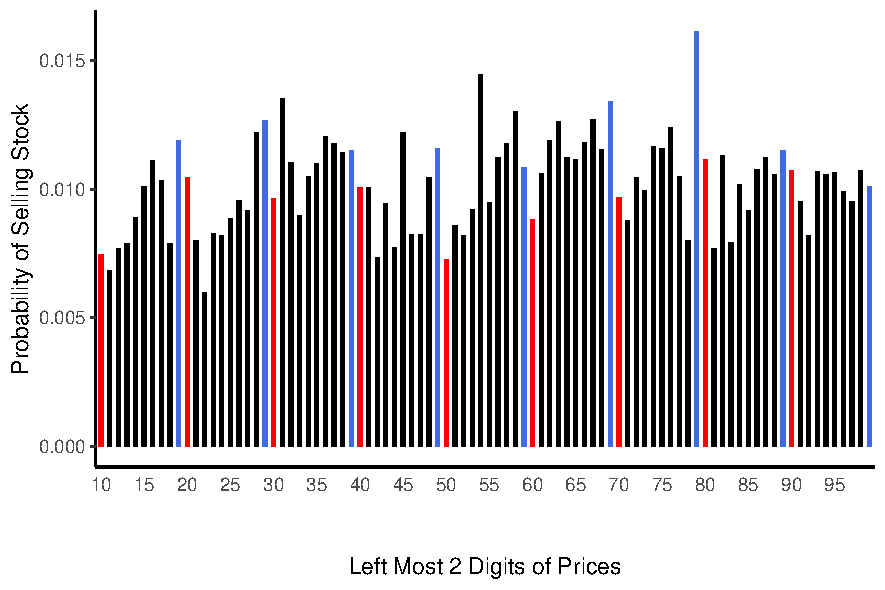
\includegraphics[width=0.45\textwidth]{figures/2left_decrease_bin1p_quarter.pdf}
	}
	\subfigure[Price = \pounds1.00 to \pounds10.0]{
		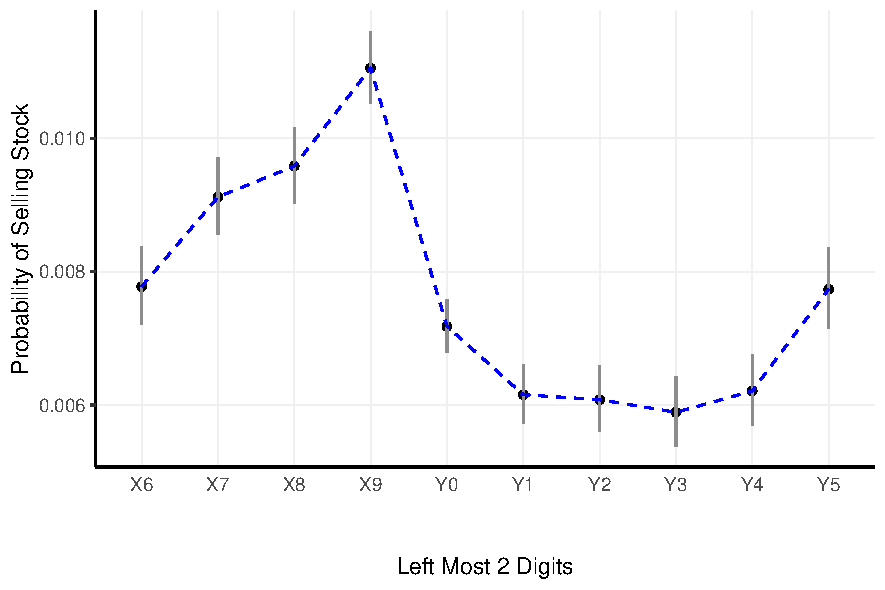
\includegraphics[width=0.45\textwidth]{figures/Left2decreases_10pbin_CI_quarter.pdf}
		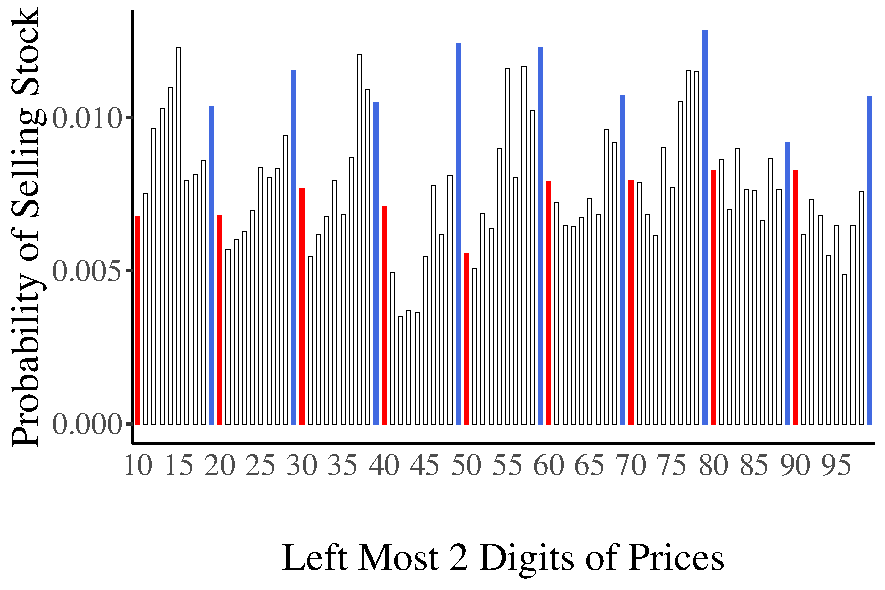
\includegraphics[width=0.45\textwidth]{figures/2left_decrease_bin10p_quarter.pdf}
	}
	\subfigure[Price = \pounds10 to \pounds100]{
		\includegraphics[width=0.45\textwidth]{figures/Left2decreases_1poundbin_CI_quarter.pdf}
		\includegraphics[width=0.45\textwidth]{figures/2left_decrease_bin1pound_quarter.pdf}
	}
	\fignote{£$Y$ in the X-axes is equivalent to £$X+1$ (e.g., £X9 could include £0.19, £1.9, £19, etc., while £Y0 could include £0.20, £2.0, £20, etc.). Panels A, B and C show equal size bins of 1p, 10p and £1, respectively. Panel A corresponds to 27\% of the observations in the prices decreasing sample; Panel B, to 43\%; and Panel C, to 7\%.}
\end{figure}

\clearpage
\begin{figure}[hbt!]
	\caption{Leftmost Stock Price Digit and Probability of Sale \\ Prices Decreasing Sample by Price Range \\ \textcolor{blue}{Sell-Price-No-Yesterday-Login, Login-Days}}%
	\label{fig:left_digit_sell_decrease_mainsss_no_yest}%
	\centering%	
	\bigskip
	\subfigure[Price = \pounds0.10 to \pounds1.00]{
		\includegraphics[width=0.45\textwidth]{figures/no_yest_loginLeft2decreases_1pbin_CI_quarter.pdf}
		\includegraphics[width=0.45\textwidth]{figures/no_yest_login2left_decrease_bin1p_quarter.pdf}
	}
	\subfigure[Price = \pounds1.00 to \pounds10.0]{
		\includegraphics[width=0.45\textwidth]{figures/no_yest_loginLeft2decreases_10pbin_CI_quarter.pdf}
		\includegraphics[width=0.45\textwidth]{figures/no_yest_login2left_decrease_bin10p_quarter.pdf}
	}
	\subfigure[Price = \pounds10 to \pounds100]{
		\includegraphics[width=0.45\textwidth]{figures/no_yest_loginLeft2decreases_1poundbin_CI_quarter.pdf}
		\includegraphics[width=0.45\textwidth]{figures/no_yest_login2left_decrease_bin1pound_quarter.pdf}
	}
	\fignote{£$Y$ in the X-axes is equivalent to £$X+1$ (e.g., £X9 could include £0.19, £1.9, £19, etc., while £Y0 could include £0.20, £2.0, £20, etc.). Panels A, B and C show equal size bins of 1p, 10p and £1, respectively. Panel A corresponds to 27\% of the observations in the prices decreasing sample; Panel B, to 43\%; and Panel C, to 7\%.}
\end{figure}

\clearpage
\begin{figure}[hbt!]
	\caption{Leftmost Stock Price Digit and Probability of Sale \\ Prices Decreasing Sample by Price Range \\ \textcolor{blue}{Sell-Price-FTSE100, Login-Days}}%
	\label{fig:left_digit_sell_decrease_mainsss_ftse}%
	\centering%	
	\bigskip
	\subfigure[Price = \pounds0.10 to \pounds1.00]{
		\includegraphics[width=0.45\textwidth]{figures/liquidLeft2decreases_1pbin_CI_quarter.pdf}
		\includegraphics[width=0.45\textwidth]{figures/liquid2left_decrease_bin1p_quarter.pdf}
	}
	\subfigure[Price = \pounds1.00 to \pounds10.0]{
		\includegraphics[width=0.45\textwidth]{figures/liquidLeft2decreases_10pbin_CI_quarter.pdf}
		\includegraphics[width=0.45\textwidth]{figures/liquid2left_decrease_bin10p_quarter.pdf}
	}
	\subfigure[Price = \pounds10 to \pounds100]{
		\includegraphics[width=0.45\textwidth]{figures/liquidLeft2decreases_1poundbin_CI_quarter.pdf}
		\includegraphics[width=0.45\textwidth]{figures/liquid2left_decrease_bin1pound_quarter.pdf}
	}
	\fignote{£$Y$ in the X-axes is equivalent to £$X+1$ (e.g., £X9 could include £0.19, £1.9, £19, etc., while £Y0 could include £0.20, £2.0, £20, etc.). Panels A, B and C show equal size bins of 1p, 10p and £1, respectively. Panel A corresponds to 27\% of the observations in the prices decreasing sample; Panel B, to 43\%; and Panel C, to 7\%.}
\end{figure}



















\appendix




\begin{econtable}[h]\small
	\caption{Sample Selection}
	\label{tab:sample_selection}
	\estauto{l c c c c c c c }{
		&\multicolumn{1}{c}{ Accounts}&\multicolumn{1}{c}{Logins}&\multicolumn{1}{c}{ Transactions}&\multicolumn{1}{c}{Sells}\\
		\midrule
		Unrestricted Sample 			&	91817	&	135331214	&	993312	\\
\textit{Drop due to:} 									\\
\hspace{0.5cm} Inactive Accounts 			&	28990	&	15951667	&	39075	\\
\hspace{0.5cm} Unmatched Prices 			&	581	&	26014606	&	101667	\\
\hspace{0.5cm} At Least Two Stocks in Portfolio		&	5999	&	1444418	&	65638	\\
\hspace{0.5cm} Missing Demographic Data 			&	2282	&	3980478	&	35724	\\
\hspace{0.5cm} Starting Position Days			&	40	&	726121	&	49899	\\
\midrule										\\
Baseline sample 			&	53925	&	87213924	&	701309	\\

	}
	\fignote{The unrestricted sample contains 155,300 accounts. We use a 30\% random sample of accounts.  The table detail the steps in sample selection. Logins, Transactions, and Sells reflect the number of observations for each category at the Account $\times$ Stock $\times$ Day level.   }
\end{econtable}

\clearpage

\begin{table}\small
	\caption{Summary Stats, Quarterly Sample \\ \textcolor{blue}{Sell-Price}}
	\label{tab:price_summary_stats_main}
	\bigskip
	\begin{adjustbox}{center}
		\estauto{lcccccccccc}<\multicolumn{9}{c}{Panel (A): Baseline Sample} \\>{
			& \multicolumn{1}{c}{N} & \multicolumn{1}{c}{Mean} & \multicolumn{1}{c}{St. Dev.} & \multicolumn{1}{c}{Min} & \multicolumn{1}{c}{Pctl(25)} & \multicolumn{1}{c}{Median} & \multicolumn{1}{c}{Pctl(75)} & \multicolumn{1}{c}{Max} \\ 	
			Price on Login Days \pounds & 43,903,112 & 7.942 & 26.178 & 0.000 & 1.153 & 3.050 & 7.642 & 15,051.630 \\ 
Price on Sell Days \pounds & 3,341,054 & 7.103 & 24.523 & 0.000 & 0.832 & 2.646 & 6.674 & 3,589.000 \\ 
Price of Stocks Sold \pounds & 342,277 & 6.848 & 16.483 & 0.000 & 0.861 & 2.714 & 6.648 & 1,771.425 \\ 
 
		}
	\end{adjustbox}
	
	\bigskip
	
	\begin{adjustbox}{center}
		\estauto{lcccccccccc}<\multicolumn{9}{c}{Panel (B): Price Increasing Sample} \\>{
			& \multicolumn{1}{c}{N} & \multicolumn{1}{c}{Mean} & \multicolumn{1}{c}{St. Dev.} & \multicolumn{1}{c}{Min} & \multicolumn{1}{c}{Pctl(25)} & \multicolumn{1}{c}{Median} & \multicolumn{1}{c}{Pctl(75)} & \multicolumn{1}{c}{Max} \\ 	
			All Stocks & 316,242 & 5.777 & 15.384 & 0.000 & 0.582 & 2.433 & 6.010 & 2,001.557 \\ 
Stocks with Prices Between \pounds 0.11 to \pounds 1.01 & 82,932 & 0.588 & 0.254 & 0.110 & 0.378 & 0.616 & 0.795 & 1.010 \\ 
Stocks with Prices Between \pounds 1.1 to \pounds 10.1 & 155,842 & 4.816 & 2.367 & 1.100 & 2.917 & 4.348 & 6.578 & 10.099 \\ 
Stocks with Prices Between \pounds 11 to \pounds 101 & 25,401 & 34.166 & 18.423 & 11.000 & 19.931 & 30.040 & 46.290 & 100.690 \\ 
 
		}
	\end{adjustbox}
	
	\bigskip
	
	\begin{adjustbox}{center}
		\estauto{lcccccccccc}<\multicolumn{9}{c}{Panel (C): Price Decreasing Sample} \\>{
			& \multicolumn{1}{c}{N} & \multicolumn{1}{c}{Mean} & \multicolumn{1}{c}{St. Dev.} & \multicolumn{1}{c}{Min} & \multicolumn{1}{c}{Pctl(25)} & \multicolumn{1}{c}{Median} & \multicolumn{1}{c}{Pctl(75)} & \multicolumn{1}{c}{Max} \\ 	
			All Stocks & 4,376,352 & 7.507 & 26.412 & 0.000 & 1.183 & 2.650 & 8.270 & 4,495.251 \\ 
Stocks with Prices Between \pounds 0.10 to \pounds 1.0 & 611,813 & 0.491 & 0.277 & 0.100 & 0.226 & 0.472 & 0.740 & 1.000 \\ 
Stocks with Prices Between \pounds 1 to \pounds 10 & 2,461,228 & 3.230 & 1.998 & 1.000 & 1.750 & 2.602 & 4.176 & 10.000 \\ 
Stocks with Prices Between \pounds 10 to \pounds 100 & 978,415 & 20.993 & 11.905 & 10.000 & 13.725 & 16.350 & 24.450 & 99.990 \\ 
 
		}
	\end{adjustbox}
\end{table}

\clearpage






\begin{figure}[hbt!]
	\centering%
	\caption{Histogram of Stock Prices}%
	\label{fig:histogram_prices}%
	\includegraphics[width=.6\textwidth]{figures/prices_hist_login_days.pdf}
	\fignote{Figure shows the histogram of prices on login days. Outliers above the 95 percentile are excluded.}
\end{figure}



%sell days


\begin{figure}[hbt!]
	\caption{Leftmost Stock Price Digit and Probability of Sale, Quarterly Sample \\ \textcolor{blue}{Market-Price, Sell-Days}}%
	\label{fig:left_digit_sell_main_market_sell}%
	\centering%	
	\bigskip %liquidLeft2increase_probCI_quarter
	\subfigure[Price Increasing]{
		\includegraphics[width=0.45\textwidth]{figures/EndDayLeft2increase_probCI_quarter_sell.pdf}
		\includegraphics[width=0.45\textwidth]{figures/EndDay2left_increase_quarter_sell.pdf}	
	}
	\subfigure[Price Decreasing]{
		\includegraphics[width=0.45\textwidth]{figures/EndDayLeft2decrease_probCI_quarter_sell.pdf}
		\includegraphics[width=0.45\textwidth]{figures/EndDay2left_decrease_quarter_sell.pdf}	
	}
	\fignote{£$Y$ in the X-axes is equivalent to £$X+1$ (e.g., £X9 could include £0.19, £1.9, £19, etc., while £Y0 could include £0.20, £2.0, £20, etc.).}
\end{figure}

\begin{figure}[hbt!]
	\caption{Leftmost Stock Price Digit and Probability of Sale, Quarterly Sample \\ \textcolor{blue}{Sell-Price, Sell-Days}}%
	\label{fig:left_digit_sell_main_sell_sell}%
	\centering%	
	\bigskip %liquidLeft2increase_probCI_quarter
	\subfigure[Price Increasing]{
		\includegraphics[width=0.45\textwidth]{figures/Left2increase_probCI_quarter_sell.pdf}
		\includegraphics[width=0.45\textwidth]{figures/2left_increase_quarter_sell.pdf}	
	}
	\subfigure[Price Decreasing]{
		\includegraphics[width=0.45\textwidth]{figures/Left2decrease_probCI_quarter_sell.pdf}
		\includegraphics[width=0.45\textwidth]{figures/2left_decrease_quarter_sell.pdf}	
	}
	\fignote{£$Y$ in the X-axes is equivalent to £$X+1$ (e.g., £X9 could include £0.19, £1.9, £19, etc., while £Y0 could include £0.20, £2.0, £20, etc.).}
\end{figure}











\begin{figure}[hbt!]
	\caption{Leftmost Stock Price Digit and Probability of Sale, Quarterly Sample \\ \textcolor{blue}{Sell-Price-No-Login-Yesterday, Sell-Days}}%
	\label{fig:left_digit_sell_main_no_yest_sell}%
	\centering%	
	\bigskip %liquidLeft2increase_probCI_quarter
	\subfigure[Price Increasing]{
		\includegraphics[width=0.45\textwidth]{figures/no_yest_loginLeft2increase_probCI_quarter_sell.pdf}
		\includegraphics[width=0.45\textwidth]{figures/no_yest_login2left_increase_quarter_sell.pdf}	
	}
	\subfigure[Price Decreasing]{
		\includegraphics[width=0.45\textwidth]{figures/no_yest_loginLeft2decrease_probCI_quarter_sell.pdf}
		\includegraphics[width=0.45\textwidth]{figures/no_yest_login2left_decrease_quarter_sell.pdf}	
	}
	\fignote{£$Y$ in the X-axes is equivalent to £$X+1$ (e.g., £X9 could include £0.19, £1.9, £19, etc., while £Y0 could include £0.20, £2.0, £20, etc.).}
\end{figure}
\begin{figure}[hbt!]
	\caption{Leftmost Stock Price Digit and Probability of Sale, Quarterly Sample \\ \textcolor{blue}{Sell-Price-FTSE100, Sell-Days}}%
	\label{fig:left_digit_sell_main_ftse_sell}%
	\centering%	
	\bigskip %liquidLeft2increase_probCI_quarter
	\subfigure[Price Increasing]{
		\includegraphics[width=0.45\textwidth]{figures/liquidLeft2increase_probCI_quarter_sell.pdf}
		\includegraphics[width=0.45\textwidth]{figures/liquid2left_increase_quarter_sell.pdf}	
	}
	\subfigure[Price Decreasing]{
		\includegraphics[width=0.45\textwidth]{figures/liquidLeft2decrease_probCI_quarter_sell.pdf}
		\includegraphics[width=0.45\textwidth]{figures/liquid2left_decrease_quarter_sell.pdf}	
	}
	\fignote{£$Y$ in the X-axes is equivalent to £$X+1$ (e.g., £X9 could include £0.19, £1.9, £19, etc., while £Y0 could include £0.20, £2.0, £20, etc.).}
\end{figure}

\clearpage



%month and year

\begin{figure}[hbt!]
	\caption{Leftmost Stock Price Digit and Probability of Sale, Monthly Sample \\ \textcolor{blue}{Market-Price, Login-Days}}%
	\label{fig:left_digit_sell_monthly_market}%
	\centering%	
	\bigskip
	\subfigure[Price Increasing]{
		\includegraphics[width=0.45\textwidth]{figures/EndDayLeft2increase_probCI_month.pdf}
		\includegraphics[width=0.45\textwidth]{figures/EndDay2left_increase_month.pdf}	
	}
	\subfigure[Price Decreasing]{
		\includegraphics[width=0.45\textwidth]{figures/EndDayLeft2decrease_probCI_month.pdf}
		\includegraphics[width=0.45\textwidth]{figures/EndDay2left_decrease_month.pdf}	
	}
	\fignote{£$Y$ in the X-axes is equivalent to £$X+1$ (e.g., £X9 could include £0.19, £1.9, £19, etc., while £Y0 could include £0.20, £2.0, £20, etc.).}
\end{figure}

\clearpage

\begin{figure}[hbt!]
	\caption{Leftmost Stock Price Digit and Probability of Sale, Annual Sample \\ \textcolor{blue}{Market-Price, Login-Days}}%
	\label{fig:left_digit_sell_annual_market}%
	\centering%	
	\bigskip
	\subfigure[Price Increasing]{
		\includegraphics[width=0.45\textwidth]{figures/EndDayLeft2increase_probCI_year.pdf}
		\includegraphics[width=0.45\textwidth]{figures/EndDay2left_increase_year.pdf}	
	}
	\subfigure[Price Decreasing]{
		\includegraphics[width=0.45\textwidth]{figures/EndDayLeft2decrease_probCI_year.pdf}
		\includegraphics[width=0.45\textwidth]{figures/EndDay2left_decrease_year.pdf}	
	}
	\fignote{£$Y$ in the X-axes is equivalent to £$X+1$ (e.g., £X9 could include £0.19, £1.9, £19, etc., while £Y0 could include £0.20, £2.0, £20, etc.).}
\end{figure}



\begin{figure}[hbt!]
	\caption{Leftmost Stock Price Digit and Probability of Sale, Monthly Sample \\ \textcolor{blue}{Sell-Price, Login-Days}}%
	\label{fig:left_digit_sell_monthly_sell}%
	\centering%	
	\bigskip
	\subfigure[Price Increasing]{
		\includegraphics[width=0.45\textwidth]{figures/Left2increase_probCI_month.pdf}
		\includegraphics[width=0.45\textwidth]{figures/2left_increase_month.pdf}	
	}
	\subfigure[Price Decreasing]{
		\includegraphics[width=0.45\textwidth]{figures/Left2decrease_probCI_month.pdf}
		\includegraphics[width=0.45\textwidth]{figures/2left_decrease_month.pdf}	
	}
	\fignote{£$Y$ in the X-axes is equivalent to £$X+1$ (e.g., £X9 could include £0.19, £1.9, £19, etc., while £Y0 could include £0.20, £2.0, £20, etc.).}
\end{figure}

\clearpage

\begin{figure}[hbt!]
	\caption{Leftmost Stock Price Digit and Probability of Sale, Annual Sample \\ \textcolor{blue}{Sell-Price, Login-Days}}%
	\label{fig:left_digit_sell_annual_sell}%
	\centering%	
	\bigskip
	\subfigure[Price Increasing]{
		\includegraphics[width=0.45\textwidth]{figures/Left2increase_probCI_year.pdf}
		\includegraphics[width=0.45\textwidth]{figures/2left_increase_year.pdf}	
	}
	\subfigure[Price Decreasing]{
		\includegraphics[width=0.45\textwidth]{figures/Left2decrease_probCI_year.pdf}
		\includegraphics[width=0.45\textwidth]{figures/2left_decrease_year.pdf}	
	}
	\fignote{£$Y$ in the X-axes is equivalent to £$X+1$ (e.g., £X9 could include £0.19, £1.9, £19, etc., while £Y0 could include £0.20, £2.0, £20, etc.).}
\end{figure}


\begin{figure}[hbt!]
	\caption{Leftmost Stock Price Digit and Probability of Sale, Monthly Sample \\ \textcolor{blue}{Sell-Price-No-Login-Yesterday, Login-Days}}%
	\label{fig:left_digit_sell_monthly_no_yest}%
	\centering%	
	\bigskip
	\subfigure[Price Increasing]{
		\includegraphics[width=0.45\textwidth]{figures/no_yest_loginLeft2increase_probCI_month.pdf}
		\includegraphics[width=0.45\textwidth]{figures/no_yest_login2left_increase_month.pdf}	
	}
	\subfigure[Price Decreasing]{
		\includegraphics[width=0.45\textwidth]{figures/no_yest_loginLeft2decrease_probCI_month.pdf}
		\includegraphics[width=0.45\textwidth]{figures/no_yest_login2left_decrease_month.pdf}	
	}
	\fignote{£$Y$ in the X-axes is equivalent to £$X+1$ (e.g., £X9 could include £0.19, £1.9, £19, etc., while £Y0 could include £0.20, £2.0, £20, etc.).}
\end{figure}

\clearpage

\begin{figure}[hbt!]
	\caption{Leftmost Stock Price Digit and Probability of Sale, Annual Sample \\ \textcolor{blue}{Sell-Price-No-Login-Yesterday, Login-Days}}%
	\label{fig:left_digit_sell_annual_no_yest}%
	\centering%	
	\bigskip
	\subfigure[Price Increasing]{
		\includegraphics[width=0.45\textwidth]{figures/no_yest_loginLeft2increase_probCI_year.pdf}
		\includegraphics[width=0.45\textwidth]{figures/no_yest_login2left_increase_year.pdf}	
	}
	\subfigure[Price Decreasing]{
		\includegraphics[width=0.45\textwidth]{figures/no_yest_loginLeft2decrease_probCI_year.pdf}
		\includegraphics[width=0.45\textwidth]{figures/no_yest_login2left_decrease_year.pdf}	
	}
	\fignote{£$Y$ in the X-axes is equivalent to £$X+1$ (e.g., £X9 could include £0.19, £1.9, £19, etc., while £Y0 could include £0.20, £2.0, £20, etc.).}
\end{figure}


\begin{figure}[hbt!]
	\caption{Leftmost Stock Price Digit and Probability of Sale, Monthly Sample \\ \textcolor{blue}{Sell-Price-FTSE100, Login-Days}}%
	\label{fig:left_digit_sell_monthly_ftse}%
	\centering%	
	\bigskip
	\subfigure[Price Increasing]{
		\includegraphics[width=0.45\textwidth]{figures/liquidLeft2increase_probCI_month.pdf}
		\includegraphics[width=0.45\textwidth]{figures/liquid2left_increase_month.pdf}	
	}
	\subfigure[Price Decreasing]{
		\includegraphics[width=0.45\textwidth]{figures/liquidLeft2decrease_probCI_month.pdf}
		\includegraphics[width=0.45\textwidth]{figures/liquid2left_decrease_month.pdf}	
	}
	\fignote{£$Y$ in the X-axes is equivalent to £$X+1$ (e.g., £X9 could include £0.19, £1.9, £19, etc., while £Y0 could include £0.20, £2.0, £20, etc.).}
\end{figure}

\clearpage

\begin{figure}[hbt!]
	\caption{Leftmost Stock Price Digit and Probability of Sale, Annual Sample \\ \textcolor{blue}{Sell-Price-FTSE100, Login-Days}}%
	\label{fig:left_digit_sell_annual_ftse}%
	\centering%	
	\bigskip
	\subfigure[Price Increasing]{
		\includegraphics[width=0.45\textwidth]{figures/liquidLeft2increase_probCI_year.pdf}
		\includegraphics[width=0.45\textwidth]{figures/liquid2left_increase_year.pdf}	
	}
	\subfigure[Price Decreasing]{
		\includegraphics[width=0.45\textwidth]{figures/liquidLeft2decrease_probCI_year.pdf}
		\includegraphics[width=0.45\textwidth]{figures/liquid2left_decrease_year.pdf}	
	}
	\fignote{£$Y$ in the X-axes is equivalent to £$X+1$ (e.g., £X9 could include £0.19, £1.9, £19, etc., while £Y0 could include £0.20, £2.0, £20, etc.).}
\end{figure}


\clearpage



\begin{onehalfspacing}
	\bibliographystyle{chicago}
	\bibliography{left_digit_bibliography}
\end{onehalfspacing}

%main figures and tables
\singlespacing

\end{document}
